\chapter{Manifold Learning}

\section{Introduction}

% Start with section on manifold learning of AD and MS
% populations. Including a summary of those methods and the whole literature
% review of what has been done. This includes manifold learning, population
% studies, disease classification and the likes without deep learning.

The need for manifold learning often arises when very high-dimensional data
needs to be analyzed but the intrinsic dimensionality of the data is much lower.
This situations occurs, for example, when trying to visualize variability and
common patterns in a given group of magnetic resonance images (MRIs) of the
brain. Each image can be regarded as a point in a high-dimensional image space
(called the ambient space), with $n_x \times n_y \times n_z$ coordinates, where
$n_x, n_y, n_z$ are the dimensions of each image. On the other hand, each image
could also be identified by a smaller set of parameters that describe shape
variations and patterns that are common for a particular group of images. These
parameters span a new space called the manifold space. The task of manifold
learning is to discover the low-dimensional space and its parameters which can
then be used to model the anatomical variability within a population.

In this chapter, we will use manifold learning to detect patterns of variability
in groups of images. Variability is captured in terms of the coordinates in
manifold space, which can be used as imaging biomarkers for assessing the
disease state or for classification into different subtypes. In this chapter, we
propose using a deep learning model called a deep belief network for learning
the manifold of medical images. The potential of deep learning for manifold
learning was evaluated on images of AD patients and MS patients.


\section{Related Work}

% TODO: Extend review

Various methods for manifold learning have been proposed (e.g., locally linear
embedding (LLE) \citep{saul2003}, Laplacian eigenmaps (LEM) \citep{belkin2002},
Isomaps \citep{tenenbaum2000}), with Isomaps and LEM being the most popular for
medical image analysis. Both methods require a prebuild proximity graph. In
order to build the proximity graph, it is assumed that the manifold space is
locally linear, which means that distances between neighboring points in
manifold space can be approximated by their distances in ambient space. Gerber
et. al. have shown that the choice of a suitable distance measure is crucial for
manifold learning using Isomaps and that the warping distance between brain
images improves the learning performance over previously used Euclidean
distances in the image space \citep{gerber2010}.

Manifolds have been used to regularize the segmentation of brain
ventricles~\citep{etyngier2007}, and to constrain the deformable registration of
brain images to have biologically plausible parameters \citep{hamm2010}. Gerber
et al. used Isomaps to predict clinical parameters of Alzheimers's (AD) patients
\citep{gerber2010}, and Wolz et al. used Laplacian eigenmaps to perform
biomarker discovery \citep{wolz2011}, also of AD patients, and atlas propagation
for the segmentation of the hippocampus \citep{wolz2010}.

\section{Deep Belief Networks for Manifold Learning of Brain MRIs}

I need to formalize manifold learning mathematically so that I have a common
notation similar to how I formalized segmentation.

One of the most important applications of deep learning is to learn a feature
hierarchy from unlabeled images. The key to learning such a hierarchy is the
ability of deep models to be trained layer by layer, where each layer acts as a
nonlinear feature extractor. Various methods have been proposed for feature
extraction from unlabeled images. In this section, we will first introduce the
restricted Boltzmann machines (RBMs) \citep{freund1992,hinton2010}, which are the
building blocks of deep belief networks (DBNs) \citep{Hinton2006b}, followed by
a short introduction to alternative feature extractors such as stacked denoising
autoencoders (SDAEs) \citep{vincent2010}.

% TODO: comparison to supervised methods similar to the introduction of the
% supervised methods section.

\subsection{From Restricted Boltzmann Machines to Deep Belief Networks}

% TODO: Illustrate with toy example.

An RBM is a probabilistic graphical models defined by a bipartite graph as shown
in Fig.~\ref{fig:rbm}. The units of the RBM are divided into two layers, one of
visible units $\vect{v}$ and the other of hidden units $\vect{h}$. There are no
direct connections between units within either layer. An RBM defines the joint
probability of visible and hidden units in terms of the energy $E$
\begin{align}
p(\vect{v}, \vect{h} \given \thetas) &=
\frac{1}{Z(\thetas)}e^{-E(\vect{v}, \vect{h} \given \thetas)}. \\
\intertext{When the visible and hidden units are binary, the energy is defined
as} 
-E(\vect{v}, \vect{h}\given \thetas) &= \sum_{i, j}v_i w_{ij} h_j +
\sum_i b_i v_i + \sum_j c_j h_j \\
&= \vect{v}^\textup{T}\vect{W}\vect{h} + \vect{b}^\textup{T}\vect{v} +
\vect{c}^\textup{T}\vect{h}
\end{align}
where $Z(\thetas)$ is a normalization constant, $\vect{W}$ denotes the weight
matrix that connects the visible units with the hidden units, $\vect{b}$ is a
vector containing the visible bias terms, $\vect{c}$ is a vector containing the
hidden bias terms, and $\thetas = \{\vect{W}, \vect{b}, \vect{c}\}$ are the
trainable parameters of the RBM.

\begin{figure}
\centering
\begin{tikzpicture}

\tikzstyle{gnode}=[shape=circle,draw=black]

\foreach \x in {1,...,3} {
  \node[gnode] (h\x) at (2*\x-4, 0) {$h_\x$};
}
\foreach \y in {1,...,5} {
  \node[gnode] (v\y) at (1.5*\y-4.5, -2) {$v_\y$};
}
\foreach \x in {1,...,3} {
  \foreach \y in {1,...,5} {
      \draw (h\x)--(v\y);
  }
}

\node[pin=120:$w_{11}$] at ($(v1)!.5!(h1)$) {};

\coordinate (rh) at (4,0);
\coordinate (rv) at (4,-2);

\node[fit=(v1)(v5)(rv),inner sep=0pt] (visibles) {};
\node[fit=(h1)(rh), inner sep=0pt] (hiddens) {};
\node[fit=(v1)(v3), inner xsep=0pt] (inputs) {};
\node[fit=(v4)(v5), inner xsep=0pt] (outputs) {};

\begin{scope}[decoration=brace]

\draw[decorate] ($(visibles.north east)-(0,2pt)$)--node[right=4pt]{Visible
units $\vect{v}$}
(visibles.south east);

\draw[decorate] (hiddens.north  east)--
node[right=4pt,align=center]{Hidden units $\vect{h}$}
($(hiddens.south east)+(0,2pt)$);

\draw[decorate] ($(hiddens.south east)-(0,2pt)$)
--node[right=4pt,align=left] {Weights $\vect{W}$ between\\ visible and
hidden units} ($(visibles.north east)+(0,2pt)$);

% \draw[decorate] (inputs.south east)--
% node[below=4pt] {Input units: $\vect{x}$}
% (inputs.south west);
% \draw[decorate] (outputs.south east)--
% node[below=4pt] {Output units: $\vect{y}$}
% (outputs.south west);
\end{scope}

\end{tikzpicture}

\caption[Graph representation of an RBM with 3 hidden and 5 visible units]{%
Graph representation of an RBM with 3 hidden and 5 visible units.
An RBM models the joint probability of visible and hidden units. Edges between
vertices denote conditional dependence between the corresponding random
variables.}
  
\label{fig:rbm}
\end{figure}

\paragraph{Inference}
The hidden units represent patterns of similarity that can be observed in groups
of images. Once an RBM is trained, the features of a previously unseen image can
be extracted by calculating the expectation of the hidden units. The posterior
distribution of the hidden units given the visible units can be calculated by
\begin{equation}
\label{eq:dhgivenv}
p(h_j = 1 \given \vect{v}, \thetas) = \sigm(\vect{w}_{\cdot,j}^\text{T}\vect{v}
+ c_j),
\end{equation}
where $\vect{w}_{\cdot,j}$ denotes the $j$th column vector of $\vect{W}$, and
$\sigm(x)$ is the sigmoid function defined as $\sigm(x) = (1+ \exp(-x))^{-1}, x
\in \R$. An RBM is a generative model, which allows for the reconstruction of
an input signal given its features. This is achieved by calculating the expectation
of the visible units given the hidden units. The posterior distribution $p(v_i =
1 \given \vect{h}, \thetas)$ can be calculated by
\begin{equation}
\label{eq:dvgivenh}
p(v_i = 1 \given \vect{h}, \thetas) = \sigm(\vect{w}_{i,
\cdot}^\text{T}\vect{h} + b_i),
\end{equation}
where $\vect{w}_{i,\cdot}$ denotes the $i$th row vector of $\vect{W}$.
Reconstructing the visible units can be used to visualize the learned features.
To visualize the features associated with a particular hidden unit, all other
hidden units are set to zero and the expectation of the visible units is
calculated, which represents the pattern that causes a particular hidden
unit to be activated.

\paragraph{Training}

% \begin{itemize}
%   \item There are different training methods for RBMs.
%   \item Will focus on constrastive divergence.
%   \item Alternatives are stochastic bla with a reference
%   \item RBMs are trained using maximum likelihood estimation (MLE)
% \end{itemize}

RBMs can be trained by maximizing the likelihood or, more commonly, the log
likelihood of the training data, $\data = \{\vect{v}_n \given n \in [1, N] \}$,
which is called maximum likelihood estimation (MLE). The gradient of the log
likelihood function with respect to the weights, $\vect{W}$, is given by
\begin{equation}
\label{eq:mle}
\nabla_{\vect{W}} \log p(\mathcal{D} \given \thetas) =
\frac{1}{N} \sum_{n = 1}^N
\E[\vect{v}\vect{h}^\text{T} \given \vect{v}_n, \thetas]
-\E[\vect{v}\vect{h}^\text{T} \given \thetas].
\end{equation}
The first expectation can be estimated using a mean field approximation:
\begin{align}
\E[\vect{v}\vect{h}^\text{T} \given \vect{v}_n, \thetas] &\approx
\E[\vect{v} \given \vect{v}_n, \thetas]
\E[\vect{h}^\text{T} \given \vect{v}_n, \thetas], \\
&=\vect{v}_n\E[\vect{h}^\text{T} \given \vect{v}_n, \thetas].
\end{align}
The second expectation is typically estimated using a Monte Carlo
approximation
\begin{equation}
\E[\vect{v}\vect{h}^\text{T} \given \thetas] \approx
\frac{1}{S}\sum_{s=1}^{S}\vect{v}_s\vect{h}_s^\text{T},
\end{equation}
where $S$ is the number of generated samples, and $\vect{v}_s$ and $\vect{h}_s$
are samples drawn from $p(\vect{v}\given \thetas)$ and $p(\vect{h}\given
\thetas)$, respectively. Samples from an RBM can be generated efficiently using
block Gibbs sampling, in which the visible and hidden units are initialized
with random values and alternately sampled given the previous state using
\begin{align}
h_j &= \I(y_j < p(h_j = 1 \given \vect{v}, \thetas)) & \text{with $y_j \sim
\text{U}(0,1)$}\\
v_i &= \I(x_i < p(v_i \given \vect{h}, \thetas)) & \text{with $x_i \sim
\text{U}(0,1)$}
\end{align}
where $z \sim \text{U}(0,1)$ denotes a sample drawn from the uniform
distribution in the interval $[0,1]$ and $\I$~is the indicator function, which
is defined as $1$ if the argument is true and $0$ otherwise. After several
iterations, a sample generated by the Gibbs chain is distributed according to
$p(\vect{vh}\given \thetas)$.

If the Gibbs sampler is initialized at a data point from the training set and
only $1$ Monte Carlo sample is used to approximate the second expectation in
\eqref{eq:mle}, the learning algorithm is called contrastive divergence (CD)
\citep{hinton2002}. Alternatively, persistent CD (PCD) \citep{tieleman2008} uses
several separate Gibbs chains to generate data independent samples from the
model, which results in a better approximation of the gradient of the log
likelihood than CD. To speed up the training, the dataset is usually divided
into small subsets called mini-batches and a gradient step is performed for each
mini-batch. To avoid confusion with a gradient step, the term ``iteration'' is
generally avoided and the term ``epoch'' is used instead to indicate a sweep
through the entire dataset. Additional tricks to monitor and speed up the
training of an RBM can be found in Hinton's RBM training guide
\citep{hinton2010a}.

\paragraph{Deep belief networks}

A single RBM can be regarded as a nonlinear feature extractor. To learn a
hierarchical set of features, multiple RBMs are stacked and trained layer by
layer, where the first RBM is trained on the input data and subsequent RBMs are
trained on the hidden unit's activations computed from the previous RBM. The
stacking of RBMs can be repeated to initialize DBNs of any depth.

\paragraph{Alternative unit types}

To model real-valued inputs like the intensities of some medical images, the
binary visible units of an RBM are replaced with Gaussian visible units, which
leads to the following energy function
\begin{equation} 
-E(\vect{v}, \vect{h}\given \boldsymbol{\theta}) = \sum_{i,
j}\frac{v_i}{\sigma_i} w_{ij} h_j + \sum_i \frac{(v_i - b_i)^2}{2\sigma_i^2} +
\sum_j c_j h_j,
\end{equation}
where the mean of the $i$th visible unit is encoded in the bias term $b_i$,
and its standard deviation is given by $\sigma_i$. Although approaches have been
proposed to learn the standard deviation \citep{cho2011}, the
training data is often simply standardized to have zero mean and unit variance,
which yields to the following simplification for the inference of the visible
and hidden units:
\begin{align} 
\label{eq:ghgivenv}
\E[h_j \given \vect{v}, \thetas] &=
\sigm(\vect{w}_{\cdot,j}^\text{T}\vect{v} + c_j),\\
\label{eq:gvgivenh}
\E[v_i \given \vect{h}, \thetas] &= \vect{w}_{i,\cdot}^\text{T}\vect{h} +
b_i.
\end{align}

A binary hidden unit can only encode two states. In order to increase the
expressive power of the hidden units, Nair et al. proposed using noisy rectified
linear units (NReLU) \citep{nair2010} as the hidden units, and showed that this
can improve the learning performance of RBMs. The signal of an NReLU is the sum
of an infinite number of binary units all of which having the same weights but
different bias terms. In the special case where the offsets of their bias
terms are set to $-0.5, -1.5, \dotsc$, the sum of their probabilities and
therefore the expectation of an NReLU is extremely close to having a closed form:
\begin{align}
\E[h_j \given \vect{v}, \thetas] &=
\sum_{i=1}^\infty \sigm(\vect{w}_{\cdot,j}^\text{T}\vect{v} + c_j - i + 0.5),\\
&\approx \log(1+\exp(\vect{w}_{\cdot,j}^\text{T}\vect{v} + c_j)).
\end{align}
However, sampling of this type of unit involves the repeated calculation of the
sigmoid function, which can be time-consuming. If a sample is not constrained
to being an integer, a fast approximation can be calculated with
\begin{align} 
h_j &\sim \max(0, \mu_j + \Norm(0, \sigm(\mu_j))), \\
\mu_j &= \vect{w}_{\cdot,j}^\text{T}\vect{v} + c_j,
\end{align}
where $\Norm(0, \sigma^2)$ denotes Gaussian noise.

\subsection{Convolutional Models}

A potential drawback of DBNs is that the learned features are location
dependent. Hence, features that can occur at many different locations in an
image, such as edges and corners, have to be relearned for every possible
location, which dramatically increases the number of features required to
capture the content of large images. To increase the translational invariance of
the learned features, Lee et al. introduced the convolutional deep belief
network (convDBN) \citep{lee2009,lee2011}. In a convDBN, the units of one layer
are only connected to the units of a sub-region of the previous layer, where
each unit shares the same weights with all other units of the same layer. This
greatly reduces the number of trainable weights, which reduces the risk of
overfitting, reduces the memory required to store the model parameters, speeds
up the training, and thereby facilitates the application to high-resolution
images.

We assume the input images to be square 2D images, but the model generalizes
with little modification to non-square images of higher dimensions.

A convDBN consists of alternating convolutional and pooling layers, which are
followed by one or more dense layers. Each convolutional layer of the model can
be trained in a greedy layerwise fashion by treating it as a convolutional
restricted Boltzmann machine (convRBM). The energy of a convRBM is defined as
\begin{align} 
E(\vect{v},\vect{h}) 
% &= -\sum_{i=0}^{N_\text{c}-1} \sum_{j=0}^{N_\text{k}-1}
% \sum_{x,y=0}^{N_\text{h}-1} \sum_{u,v=0}^{N_\text{w}-1} h_{xy}^jw_{uv}^{ij}v_{x+u, y+v}^i
% - \sum_{i=0}^{N_\text{c}-1}b_i\!\sum_{x,y = 0}^{N_\text{v}-1}\!v_{xy}^i
% - \sum_{j=0}^{N_\text{k}-1}c_j\!\sum_{x,y = 0}^{N_\text{h}-1}\!h_{xy}^j \\
&= -\sum_{i=1}^{N_\text{c}} \sum_{j=1}^{N_\text{k}} \vect{h}^{(j)}
\bullet (\tilde{\vect{w}}^{(ij)} * \vect{v}^{(i)}) -
\sum_{i=1}^{N_\text{c}}b_i\sum_{x,y = 1}^{N_\text{v}}\!v_{xy}^{(i)} -
\sum_{j=1}^{N_\text{k}}c_j\sum_{x,y = 1}^{N_\text{h}}\!h_{xy}^{(j)}.
\end{align}
The key terms and notation are defined in Table~\ref{tab:notation}. At the first
layer, the number of channels $N_\text{c}$ is equal to the number of input
modalities. For subsequent layers, $N_\text{c}$ is equal to the number of
filters of the previous layer.

\begin{table} 
\caption{Key variables and notation. For notational simplicity,
we assume the input images to be square 2D images.}
\label{tab:notation}
\begin{center}
\begin{tabular}{@{}cL{10cm}@{}}
\toprule
Symbol & Description \\
\cmidrule(r){1-1}\cmidrule(l){2-2}
$\vect{v}^{(i)}$ & $i$th input channel \\
$\vect{h}^{(j)}$ & $j$th output channel or feature map \\
$\vect{w}^{(ij)}$ & weights of filter kernels connecting visible units
$\vect{v}^{(i)}$ to hidden units $\vect{h}^{(j)}$ \\
$b_i$ & bias terms of visible units \\
$c_j$ & bias terms of hidden units \\
$N_\text{c}$ & number of channels of the visible units \\
$N_\text{v}^2$ & number of visible units per channel \\
$N_\text{k}$ & number of filters and feature maps \\
$N_\text{h}^2$ & number of hidden units per feature map \\
%$N_\text{w}^2$ & number of weights per filter kernel \\
$\bullet$ & element-wise product followed by summation \\
$*$ & valid convolution \\
$\circledast$ & full convolution \\
$\tilde{\vect{w}}^{(ij)}$ & horizontally and vertically flipped version of
$\vect{w}^{(ij)}$ \\
\bottomrule
\end{tabular}
\end{center}
\end{table}
The posterior distributions $p(\vect{h} \given \vect{v})$ and $p(\vect{v} \given
\vect{h})$ can be derived from the energy equation and are given by
\begin{align}
p(h_{xy}^{(j)} = 1 \given \vect{v}) &= \sigm\Big(\sum_{i=0}^{N_\text{c}-1}
(\tilde{\vect{w}}^{(ij)}*\vect{v}^{(i)})_{xy} + c_j\Big), \\ 
p(v_{xy}^{(i)} = 1 \given \vect{h}) &= \sigm\Big(\sum_{j=0}^{N_\text{k}-1}
(\vect{w}^{(ij)} \circledast \vect{h}^{(j)})_{xy} + b_i\Big).
\end{align}
To train a convRBM on a set of images $\data = \{\vect{v}_n \given n \in
[1,N]\}$, the weights and bias terms can be learned by CD. During each iteration
of the algorithm, the gradient of each parameter is estimated and a gradient
step with a fixed learning rate is applied. The gradient of the filter weights
can be approximated by
\begin{equation}
\Delta \vect{w}^{(ij)} \approx
\frac{1}{N}(\vect{v}^{(i)}_n*\tilde{\vect{h}}^{(j)}_n -
\vect{v}'^{(i)}_n*\tilde{\vect{h}}_n'^{(j)}),
\label{eq:convgra}
\end{equation}
where $\vect{h}_n^{(j)}$ and $\vect{h}'^{(j)}_n$ are samples drawn from
$p(\vect{h}^{(j)} \given \vect{v}_n)$ and $p(\vect{h}^{(j)} \given
\vect{v}'_n)$, and $\vect{v}'^{(i)}_n = \E[\vect{v}^{(i)} \given \vect{h}_n]$.

Different types of operations \citep{scherer2010} have been
proposed for the pooling layers, with the common goal of creating a more compact
representation of the input data. The most commonly used type of pooling is
max-pooling. Therefore, the input to the pooling layer is divided into small
blocks and only the maximum value of each block as passed on to the next layer,
which makes the representation of the input invariant to small
translations in addition to reducing its dimensionality.

\subsection{Strided Convolutional Models}

% Why strided! Less memory, faster, no pooling required. Better correspondence
% to dense DBNs. Draw from the journal paper.

Strided convolutions are a type of convolution that shifts the filter kernel as
a sliding window with a step size or stride $s > 1$, stopping at only $N_\text{v}
/ s$ positions. This reduces the number of hidden units per channel to
$N_\text{h} = N_\text{v} / s$, hence significantly reducing training times and
memory required for storing the hidden units during training. The energy of a
strided convolutional RBM (sconvRBM) is defined as
\begin{equation} 
E(\vect{v},\vect{h}) = 
-\sum_{i=0}^{N_\text{c}-1}\sum_{j=0}^{N_\text{k}-1}\sum_{x,y=0}^{N_\text{h}-1}
\sum_{u,v=-\lfloor N_\text{w}/2\rfloor}^{\lfloor(N_\text{w}-1)/2\rfloor}
\hspace{-1.2em}h_{xy}^jw_{uv}^{ij}v_{sx+u, sy + v}^i -
\sum_{i=0}^{N_\text{c}-1}b_i\!\sum_{x,y = 0}^{N_\text{v}-1}\!v_{xy}^i -
\sum_{j=0}^{N_\text{k}-1}c_j\!\sum_{x,y = 0}^{N_\text{h}-1}\!h_{xy}^j
\end{equation}  

\section{Training of Deep Belief Networks}

Deep learning has traditionally been computationally expensive and advances in
training methods have been the prerequisite for expanding its application to a
variety of image classification problems. The development of layer-wise training
methods \citep{Hinton2006b} greatly improved the efficiency of the training of
deep belief networks (DBNs), which has made feasible the use of large sets of
small images (e.g. \num{28x28}), such as those used for hand-written digit
recognition. Subsequently, new directions for speeding up the training of deep
models were opened with the advance of programmable graphics cards (GPUs), which
can perform thousands of operations in parallel. \Citet{Raina2009} demonstrated
that by using graphics cards, training of restricted Boltzmann machines (RBMs)
on small image patches (e.g. \num{24x24}) can be performed up to \num{70} times
faster than on the CPU, facilitating the application to larger training sets.
However, the number of trainable weights of a DBN increases greatly with the
resolution of the training images, which can make training on large images
impracticable. In order to scale DBNs to high-resolution images,
\citet{lee2009,lee2011} introduced the convolutional deep belief network
(convDBN), a deep generative model that uses weight sharing to reduce the number
of trainable weights. They showed that a convDBN can be used to classify images
with a resolution up to \num{200x200} pixels. To speed up the training of
convolutional neural networks (CNNs) on high-resolution images,
\citet{Krizhevsky2012} replaced traditional convolutions of the first layer of
their CNN with strided convolutions, a type of convolution that shifts the
filter kernel as a sliding window with a fixed step size or stride greater than
one. Through the use of strided convolutions, the number of hidden units in each
convolutional layer is greatly reduced, which reduces both training time and
required memory. Using a highly optimized GPU implementation of convolutions,
they were able to train a CNN on images with a resolution of \num{256x256}
pixels, achieving state-of-the-art performance on the ILSVRC-2010 and
ILSVRC-2012 competitions \citep{Krizhevsky2012}. An alternative approach was
proposed by \citet{Mathieu2013} who sped up the training of CNNs by calculating
convolutions between batches of images and filters using fast Fourier transforms
(FFTs), albeit at the cost of additional memory required for storing the
filters.

In this paper, we detail our training algorithm and GPU implementation in full,
with a much more thorough analysis of the running time on high-resolution 2D
images (\num{512x512}) and 3D volumes (\num{128x128x128}), showing speed-ups of
up to 8-fold and 200-fold, respectively. Our proposed method performs training
in the frequency domain, which replaces the calculation of time-consuming
convolutions with simple element-wise multiplications, while adding only a small
number of FFTs. In contrast to similar FFT-based approaches
\citep[e.g.,][]{Mathieu2013}, our method does not use batch processing of the
images as a means to reduce the number of FFT calculations, but rather minimizes
FFTs even when processing a single image, which significantly reduces the
required amount of scarce GPU memory. We show that our method can be efficiently
implemented on multiple graphics cards, further improving the runtime
performance over other GPU-accelerated training methods. In addition, we
formalize the expression of the strided convolutional DBN (sconvDBN), a type of
convDBN that uses strided convolutions to speed up training and reduce memory
requirements, in terms of stride-1 convolutions, which enables the efficient
training of sconvDBNs in the frequency domain.

% TODO: Follow up with how to train them in the medical domain.
% Introduction and motivation. Talks about special challenges. Training in the
% frequency domain is important and a main contribution of this thesis. This will
% be about my algorithm, how it works for convRBMs and CNNs. Especially the tricks
% needed for strided convolutions.

% Mapping in the frequency domain. Minimize transforms. Also memory
% considerations and the likes. Also trick to do strided convolutions in the
% frequency domain.

\subsection{Training of convDBNs in the Spatial Domain}

% Short revision of how training works. Put all the pieces together to make it
% an algorithm. Make sure that I do this for convRBMs

To train an sconvRBM on a set of images, the
weights and bias terms can be learned by CD. During each iteration of the
algorithm, the gradient of each parameter is estimated and a gradient step with
a fixed learning rate is applied. The gradient of the filter weights can be
approximated by
\begin{equation}
\Delta \vect{W}^{ij} \approx \frac{1}{N}(\vect{V}^i_n*\tilde{\vect{h}}^j_n -
\vect{V}'^i_n*\tilde{\vect{h}}_n'^j)
\label{eq:convgra}
\end{equation}
where $\vect{V}_n, n \in [0,N-1]$ are reindexed images from the training set,
$\vect{h}_n^j$ and $\vect{h}'^j_n$ are samples drawn from $p(\vect{h}^j \given
\vect{V}_n)$ and $p(\vect{h}^j \given \vect{V}'_n)$, and $\vect{V}'^i_n =
\E[\vect{V}^i \given \vect{h}_n]$.
To apply the model to real-valued data like certain types of images, the
visible units can be modeled as Gaussian units. When the visible units are
mean--centered and standardized to unit variance, the expectation of the visible
units is given by
\begin{equation} 
\E[\vect{V}^i \given \vect{h}] = \textstyle\sum_j \vect{W}^{ij}*\vect{h}^j + b_i
\label{eq:convvis}
\end{equation}
A binary hidden unit can only encode two states. In order to increase the
expressive power of the hidden units, we use noisy rectified linear units as the
hidden units, which have been shown to improve the learning performance
of RBMs \citep{Nair2010}. The hidden units can be sampled with
\begin{align} 
\vect{h}^j &\sim \max(0, \mu^j + \Norm(0, \sigm(\mu^j))) \\
\mu^j &= \textstyle\sum_i\tilde{\vect{W}}^{ij}*\vect{V}^i +c_j
\label{eq:convhid}
\end{align} 
where $\Norm(0, \sigma^2)$ denotes Gaussian noise. The learning algorithm in the
spatial domain is summarized in Figure~\ref{alg:spatial}.

\begin{figure}[t!]
\hspace{-1.75em}
\subfloat[Training in the spatial domain]{
\label{alg:spatial}
\begin{minipage}{0.495\linewidth}
\footnotesize
\begin{algorithm}[H]
\setstretch{1.25}
%\renewcommand{\baselinestretch}{1.25}
%\selectfont
\SetKwInOut{Input}{input}
\SetKwInOut{Output}{output}
\Input{Images $\data = \{\vect{V}_n \given n \in [0, N-1]\}$}
\Output{Weights gradient $\Delta \vect{W}$}
$\Delta \vect{W} = 0$\;
\ForEach{image $\vect{V} \in \data$} {
  $\vect{V}' = 0$\;
  \For{$j = 0$ \KwTo $N_\text{k}-1$} {
    $\mu^j = \sum_i \tilde{\vect{W}^{ij}} * \vect{V}^i + c_j$\;
    \mbox{}\\
    \BlankLine
    $h^j \sim \max(0, \mu^j + \Norm(0, \sigm(\mu^j)))$\;
    \mbox{}\\
    \For{$i = 0$ \KwTo $N_\text{C}-1$} {
      $\Delta \vect{W}^{ij} = \Delta \vect{W}^{ij} + \tilde{\vect{h}}^j *
      \vect{V}^i$\;
      $\vect{V}'^i = \vect{V}'^i + \vect{W}^{ij} * \vect{h}^j$\;
    }
  }
  $\forall i \colon \vect{V}'^i = \vect{V}'^i + b_i$\;
  \For{$j = 0$ \KwTo $N_\text{k}-1$} {
    $\mu'^j = \sum_i \tilde{\vect{W}^{ij}} * \vect{V}'^i + c_j$\;
    \mbox{}\\
    $\vect{h}'^j \sim \max(0, \mu'^j +$\\ \hfill $\Norm(0, \sigm(\mu^j)))$\;
    \mbox{}\\
    \For{$i = 0$ \KwTo $N_\text{C}-1$} {
      $\Delta \vect{W}^{ij} = \Delta \vect{W}^{ij} - \tilde{\vect{h}}'^j *
      \vect{V}'^i$\;
    }
  }
}
\end{algorithm}
\end{minipage}
}
\subfloat[Training in the frequency domain]{
\label{alg:frequency}
\begin{minipage}{0.495\linewidth}
\footnotesize
\begin{algorithm}[H]
\setstretch{1.25}
%\renewcommand{\baselinestretch}{1.25}
%\selectfont
\SetKwInOut{Input}{input}
\SetKwInOut{Output}{output}
\Input{Images $\hat{\data} = \{\hat{\vect{V}}_n \given n \in [0, N-1]\}$}
\Output{Weights gradient $\Delta\hat{\vect{W}}$}
$\Delta\hat{\vect{W}} = 0$\;
\ForEach{image $\hat{\vect{V}} \in \hat{\data}$} {
  $\hat{\vect{V}}' = 0$\;
  \For{$j = 0$ \KwTo $N_\text{k} - 1$} {
    $\hat{\mu}^j = \sum_i \overline{\hat{\vect{W}}^{ij}} \cdot
    \hat{\vect{V}}^i$\; $\mu^j = \ifft(\hat{\mu}^j) + c_j$\;
    $\vect{h}^j \sim \max(0, \mu^j + \Norm(0, \sigm(\mu^j)))$\;
    $\hat{\vect{h}}^j = \fft(\vect{h}^j)$\;
    \For{$i = 0$ \KwTo $N_\text{C}-1$} {
      $\Delta\hat{\vect{W}}^{ij} = \Delta\hat{\vect{W}}^{ij} +
      \overline{\hat{\vect{h}}^j} \cdot \hat{\vect{V}}^i$\;
      $\hat{\vect{V}}'^i = \hat{\vect{V}}'^i + \hat{\vect{W}}^{ij} \cdot
      \hat{\vect{h}}^j$\;
    }
  }
  $\forall i \colon \hat{V}_{0,0}'^i = \hat{V}_{0,0}'^i +
  N_\text{V}^2b_i$\;
  \For{$j = 0$ \KwTo $N_\text{k}-1$} {
    $\hat{\mu}'^j = \sum_i \overline{\hat{\vect{W}}^{ij}} \cdot
    \hat{\vect{V}}'^i$\;
    $\mu'^j = \ifft(\hat{\mu}'^j) + c_j$\;
    $\vect{h}'^j \sim \max(0, \mu'^j +$ \\ \hfill $\Norm(0, \sigm(\mu^j)))$\;
    $\hat{\vect{h}}'^j = \fft(\vect{h}'^j)$\;
    \For{$i = 0$ \KwTo $N_\text{C}-1$} {
      $\Delta\hat{\vect{W}}^{ij} = \Delta\hat{\vect{W}}^{ij} -
      \overline{\hat{\vect{h}}'^j} \cdot \hat{\vect{V}}'^i$\;
    }
  }
}
\end{algorithm}
\end{minipage}
}
\caption[Comparison of training algorithms of convRBMs in the
spatial and frequency domain]{Comparison of training algorithms of convRBMs in
(a) the spatial and (b) the frequency domain. Training in the frequency domain replaces the $5N_\text{k}N_\text{C}$ convolutions required in the spatial domain with simple
element-wise multiplications, while adding only $4N_\text{k}$ Fourier
transforms. The other operations are equivalent in both domains.}
\label{fig:algorithms}
\end{figure}

\subsection{Training of convDBNs in the Frequency Domain}

The computational bottleneck of the training algorithm in the spatial domain is
the calculation of convolutions, which needs to be performed $5 \times
N_\text{C} \times N_\text{k}$ times per iteration. To speed up the calculation
of convolutions, we perform training in the frequency domain, which maps the
convolutions to simple element-wise multiplications. This is especially
important for the training on 3D images due to the relatively large number of
weights of a 3D kernel compared to 2D. To minimize the number of Fourier
transforms, we map all operations needed for training to the frequency domain
whenever possible, which allows the training algorithm to stay almost entirely
in the frequency domain. All of the scalar operations needed for training
(multiplications and additions) can be readily mapped to the frequency domain
because the Fourier transform is a linear operation. Another necessary operation
is the flipping of a convolutional kernel $\tilde{w}(a) = w(-a)$, which can be
expressed by element-wise calculation of the complex conjugate; this follows
directly from the time-reversal property of the Fourier transform and the
reality condition $\hat{f}(-\xi)=\overline{\hat{f}(\xi)}$. Using the
aforementioned mappings, equations \eqref{eq:convgra} to \eqref{eq:convhid} can
be rewritten as
\begin{align}
\Delta \hat{\vect{W}}^{ij} &= \hat{\vect{V}}^i\cdot\overline{\hat{\vect{h}}^j}
- \hat{\vect{V}}'^i \cdot \overline{\hat{\vect{h}}'^j} \\
\E[\hat{V}_{xy}^i \given \vect{\hat{h}}] &=
\begin{dcases}
\textstyle\sum_j\hat{W}_{xy}^{ij}\hat{h}_{xy}^j + N_\text{V}^2 b_i &
\text{for } x,y = 0
\\
\textstyle\sum_j\hat{W}_{xy}^{ij}\hat{h}_{xy}^j & \text{for } x,y \neq 0
\end{dcases} \\
\hat{\vect{h}}^j &\sim \F\left(\max(0, \F^{-1}(\hat{\mu}^j) + c_j + 
\Norm(0, \sigma^2))\right) \\
\hat{\mu}^j
&=\textstyle\sum_i\overline{\hat{\vect{W}}^{ij}}\cdot\hat{\vect{V}}^i
\end{align}
where $\sigma^2 = \sigm(\F^{-1}(\hat{\mu}^j)+c_j)$, $\hat{x} = \F(x)$ denotes
$x$ in the frequency domain, $\F^{-1}$ denotes the inverse Fourier transform,
and $\cdot$ denotes element-wise multiplication. The algorithm for approximating the
gradient in the frequency domain is summarized in Figure~\ref{alg:frequency}.

The only operations that cannot be directly mapped to the frequency domain are
the calculation of the maximum function, the generation of Gaussian noise, and
trimming of the filter kernels. To perform the first two operations, an image
needs to be mapped to the spatial domain and back. However, these operations
need only be calculated $2N_\text{k}$ times per iteration and are therefore not
a significant contributor to the total running time. Because filter kernels are
padded to the input image size, the size of the learned filter kernels must be
explicitly enforced by trimming. This is done by transferring the filter kernels
to the spatial domain, setting the values outside of the specified filter kernel size
to zero, and then transforming the filter kernels back to the frequency domain.
This procedure needs to be performed only once per mini-batch. Since the number
of mini-batches is relatively small compared to the number of training images,
trimming of the filter kernels also does not add significantly to the total
running time of the training algorithm.

\subsection{GPU Implementation and Memory Considerations}

To further reduce training times, the algorithm can be efficiently implemented
on graphics cards, which can perform hundreds of operations in parallel.
To optimize efficiency, it is crucial to maximize the utilization of the large
number of available GPU cores, while minimizing the required amount of GPU
memory. Because our algorithm requires only a relatively small number of FFT
calculations per iteration, the computational bottleneck is the calculation of
the element-wise operations, which can be performed in parallel. Thus we
distribute the processing of a single 2D image over $N_\text{V}(\lfloor
N_\text{V}/2 \rfloor + 1) \times N_\text{C}$ independent threads, with one
thread per element in the frequency domain. The large number of parallel threads
results in a high utilization of the GPU, even when each image of a mini-batch
is processed sequentially, which we do in our method because this greatly
reduces the amount of GPU memory required to store the visible and hidden units
compared to processing batches of images in parallel.

Due to the relatively small amount of GPU memory compared to CPU memory, memory
requirements are an important consideration when designing a GPU algorithm.
However, the total amount of required memory is highly implementation-dependent
(e.g. the use of temporary variables for storing intermediate results) and a
comparison can only be done with common elements at the algorithmic level.
Therefore, in the remainder of this section, we focus on the memory requirements
of key variables such as the visible units, the hidden units, and the filters,
which are required by all implementations. In our training algorithm, all key
variables are stored in the frequency domain, where each element in the
frequency domain is represented by a single-precision complex number. Due to the
symmetry of the Fourier space, the number of elements that need to be stored is
roughly half the number of elements in the spatial domain. Thus, the memory
required for storing the visible and hidden units in the frequency domain is
roughly the same as in the spatial domain. A potential drawback of training in
the frequency domain is that the filters need to be padded to the size of the
visible units before applying the Fourier transformation, which increases the
memory required for storing the filters on the GPU. The total amount of memory
in bytes required for storing the visible units, hidden units, and padded
filters is given by the sum of their respective terms
\begin{equation} 
%\text{memory}_{\text{freq}} &= 8N_\text{v}(\lfloor N_\text{v}/2 \rfloor +1)
%\times (N_\text{c} + N_\text{k} + N_\text{k}N_\text{c}) \\
%&\approx 4N_\text{v}^2 \times (N_\text{c} + N_\text{k} + N_\text{k}N_\text{c})
% \\
% &\approx 
4N_\text{v}^2N_\text{c} + \frac{4N_\text{v}^2 N_\text{k}}{s^2} +
4N_\text{v}^2N_\text{k}N_\text{c}
\end{equation}
As a comparison, the training method of \cite{Krizhevsky2012} processes batches
of images in order to fully utilize the GPU, which requires the storing of
batches of visible and hidden units. The memory needed for storing the key
variables is given by
\begin{equation} 
%\text{memory}_{\text{spat}}= 4N_\text{v}^2 \times (N_\text{b}N_\text{c} +
% N_\text{b}N_\text{k}) + 4N_\text{w}^2N_\text{k}N_\text{c}
4N_\text{v}^2 N_\text{b}N_\text{c} + \frac{4N_\text{v}^2
N_\text{b}N_\text{k}}{s^2} + 4N_\text{w}^2N_\text{k}N_\text{c}
\end{equation}
where $N_\text{b}$ is the number of images per mini-batch. Depending on the
choice of the batch size, this method requires more memory for storing the
visible and hidden units, while requiring less memory for storing the filters.
Alternatively, \citet{Mathieu2013} proposed to speed up the training of CNNs by
calculating convolutions between batches of images and filters using FFTs. The
memory required for storing the visible units, hidden units, and filters using
this method is given by
\begin{equation}
%\text{memory}_{\text{freq}} &= 8 N_\text{v}(\lfloor N_\text{v}/2 \rfloor +1)
%\times (N_\text{b}N_\text{c} + N_\text{b}N_\text{k} + N_\text{k}N_\text{c}) \\
%&\approx 
4 N_\text{v}^2 N_\text{b}N_\text{c} + 4
N_\text{v}^2 N_\text{b}N_\text{k} + 4 N_\text{v}^2 N_\text{k}N_\text{c}
\end{equation}
Table~\ref{tab:memory} shows a comparison of the memory per GPU required for
storing key variables when training a network used in previous work by
\citet{Krizhevsky2012}. For the first layer, a comparison with Mathieu et al.'s
training method could not be performed, because that method does not support
strided convolutions, which would significantly reduce the memory required for
storing the hidden units. In all layers, the proposed approach compensates for
the increased memory requirements for the filters by considering one image at a
time rather than a batch, and still outperforms batched learning in the spatial
domain in terms of speed (see Section 3), despite not using batches.

% In all layers, the additional memory required for
% storing the padded filters is smaller than the memory required for storing
% batches of visible and hidden units. Thus, our method requires less memory for
% storing the key variables during training than two state-of-the-art
% GPU-accelerated methods.

\begin{table}[tb]

\caption[Comparison of the memory required for storing key variables using
different training methods]{Comparison of the memory required for storing key
variables using different training methods: our method (Freq), Krizhevsky et
al.'s spatial domain method (Spat), and Mathieu et al.'s method using batched
FFTs (B-FFT). A comparison with Mathieu et al.'s method could not be made for
the first layer, because that method does not support strided convolutions. In
all layers, our method consumes less memory for storing the key variables than
the other two methods.}

\label{tab:memory}
\centering
\sisetup{
  round-mode = places,
  round-precision = 1,
  exponent-product = \cdot,
  detect-weight=true,
  detect-inline-weight=math,
  tight-spacing = false,
  table-align-text-post = false
}%
\begin{tabular}{l
S[table-format=3.0]
S[table-format=3.0]
S[table-format=3.0]
S[table-format=2.0]
S[table-format=3.0]
S[table-format=1.0]
S[table-format=2.1]
S[table-format=3.1]
S[table-format=3.1]}
\toprule
Layer & {$N_\text{b}$} & {$N_\text{v}$} & {$N_\text{c}$} & {$N_\text{w}$} &
{$N_\text{k}$} & {$s$} & \multicolumn{3}{c}{Memory in MB} \\
& & & & & & & {Freq} & {Spat} & {B-FFT}
%{Out Method} & {\citet{Krizhevsky2012}} & {\cite{Mathieu2013}}
\\
\midrule
%1 (without striding) & 128 & 224 & 3 & 11 & 48 & 4 & 37.32422 & 1249.566 &
%1277.062 \\
1 & 128 & 224 & 3 & 11 & 48 & 4 & 28.71094 & 147.0665 & {---} \\
2 & 128 & 55 & 48 & 5 & 128 & 1 & 72.92938 & 260.5469 & 330.8594 \\
3 & 128 & 27 & 128 & 3 & 192 & 1 & 69.23364 & 114.75 & 182.25 \\
4 & 128 & 13 & 192 & 3 & 192 & 1 & 24.01318 & 32.95312 & 55.45312 \\
5 & 128 & 13 & 192 & 3 & 128 & 1 & 16.05005 & 27.25 & 42.25 \\
%\addlinespace
%Total & & & & & & & 210.9372 & 582.5665 & 330.8594 \\
\bottomrule
\end{tabular}\\[0.2em]
\end{table}

\subsection{Mapping Strided Convolutions to Stride-1 Convolutions}

Strided convolutions are a type of convolution that shifts the filter kernel as
a sliding window with a step size or stride $s > 1$, stopping at only $N_\text{v}
/ s$ positions. This reduces the number of hidden units per channel to
$N_\text{h} = N_\text{v} / s$, hence significantly reducing training times and
memory required for storing the hidden units during training. The energy of a
strided convolutional RBM (sconvRBM) is defined as
\begin{equation} 
E(\vect{v},\vect{h}) = 
-\sum_{i=0}^{N_\text{c}-1}\sum_{j=0}^{N_\text{k}-1}\sum_{x,y=0}^{N_\text{h}-1}
\sum_{u,v=-\lfloor N_\text{w}/2\rfloor}^{\lfloor(N_\text{w}-1)/2\rfloor}
\hspace{-1.2em}h_{xy}^jw_{uv}^{ij}v_{sx+u, sy + v}^i -
\sum_{i=0}^{N_\text{c}-1}b_i\!\sum_{x,y = 0}^{N_\text{v}-1}\!v_{xy}^i -
\sum_{j=0}^{N_\text{k}-1}c_j\!\sum_{x,y = 0}^{N_\text{h}-1}\!h_{xy}^j
\end{equation}  

\begin{figure}[tb]
\centering
\begin{tikzpicture}[node distance=0.9cm and 4.5cm]

\tikzstyle{every node}+=[font=\scriptsize\sffamily]
\tikzstyle{label}=[font=\footnotesize\sffamily]
\tikzstyle{lines}=[dashed,opacity=0]
\tikzstyle{mymatrix}=[%
  matrix of nodes,%
  inner sep=0pt,
  nodes={inner sep=2pt},
  %draw,%
  left delimiter  = (,%
  right delimiter = )%
]

\tikzstyle{every pin}+=[inner sep=2pt,align=center,pin
distance=0.1cm,font=\footnotesize\sffamily]

% \matrix [mymatrix] (image) {
% |[red]|4  & |[green]|5  & |[red]|1  & |[green]|2  & |[red]|1  & |[green]|2  \\
% |[blue]|4 & |[yellow]|2 & |[blue]|5 & |[yellow]|1 & |[blue]|1 & |[yellow]|2 \\
% |[red]|4  & |[green]|5  & |[red]|1  & |[green]|2  & |[red]|1  & |[green]|2  \\
% |[blue]|4 & |[yellow]|2 & |[blue]|5 & |[yellow]|1 & |[blue]|1 & |[yellow]|2 \\
% |[red]|4  & |[green]|5  & |[red]|1  & |[green]|2  & |[red]|1  & |[green]|2  \\
% |[blue]|4 & |[yellow]|2 & |[blue]|5 & |[yellow]|1 & |[blue]|1 & |[yellow]|2 \\
% };

\matrix [mymatrix] (image) {
4 & 2 & 1 & 8 & 2 & 7 \\
4 & 2 & 3 & 4 & 3 & 1 \\
3 & 4 & 5 & 5 & 1 & 2 \\
7 & 5 & 1 & 2 & 2 & 3 \\
2 & 1 & 2 & 2 & 7 & 5 \\
6 & 9 & 5 & 4 & 6 & 6 \\
};

\matrix [mymatrix, below=of image] (kernel) {
0.1 & -0.1 & 0.3 & 0.4 \\
0.2 & -0.3 & 0.1 & 0.1 \\
-0.4 & 0.2 & 0.2 & -0.3 \\
0.5 & -0.2 & -0.2 & 0.4 \\
};

\matrix [mymatrix, below=of kernel,thick] (map) {
%\matrix [mymatrix, above=of image,thick] (map) {
|[red]|\bfseries 6.8 & |[blue]|\bfseries 2  \\
\bfseries 4.6 &  \bfseries 3.6 \\
};

\node[fit=(image-1-1)(image-4-4), xshift=-0.5pt, yshift=-0.5pt, draw=red,inner
sep=0,thick] (window1) {};

\node[fit=(image-1-3)(image-4-6), xshift=0.5pt, yshift=0.5pt, draw=blue,inner
sep=0,thick,pin=45:{Sliding filter\\ window}] (window2) {};

\draw[decorate,decoration={brace,raise=1pt}] (window1.north
west|-window2.north west)--node[above=3pt,fill=white,fill opacity=0.5,text
opacity=1,font=\small]{$s$}(window2.north west);

\begin{pgfonlayer}{background}
\foreach \x in {1,3,5} {
  \foreach \y in {1,3,5}
    \node[fit=(image-\x-\y),inner sep=0, fill=red!15] {};
  \foreach \y in {2,4,6}
    \node[fit=(image-\x-\y),inner sep=0, fill=green!15] {};
}
\foreach \x in {2,4,6} {
  \foreach \y in {1,3,5}
    \node[fit=(image-\x-\y),inner sep=0, fill=blue!15] {};
  \foreach \y in {2,4,6}
    \node[fit=(image-\x-\y),inner sep=0, fill=yellow!30] {};
}
\foreach \x in {1,3} {
  \foreach \y in {1,3}
    \node[fit=(kernel-\x-\y),inner sep=0, fill=red!15] {};
  \foreach \y in {2,4}
    \node[fit=(kernel-\x-\y),inner sep=0, fill=green!15] {};
}
\foreach \x in {2,4} {
  \foreach \y in {1,3}
    \node[fit=(kernel-\x-\y),inner sep=0, fill=blue!15] {};
  \foreach \y in {2,4}
    \node[fit=(kernel-\x-\y),inner sep=0, fill=yellow!30] {};
}
\end{pgfonlayer}

\node[align=center] at ($(image.south)!0.5!(kernel.north)$) {\footnotesize $*$\\
(with a step size of $s$)};

%\node at ($(image.north)!0.5!(map.south)$) {$=$};
\node[label] at ($(kernel)!0.65!(map)$) {$=$};

\begin{scope}[on grid,node distance=2cm and 1.95cm] 
\matrix [mymatrix, right=3.8cm of image,fill=red!15] (image1) {
4 & 1 & 2 \\
3 & 5 & 1 \\
2 & 2 & 7 \\
};

\matrix [mymatrix, right=of image1,fill=green!15] (image2) {
2 & 8 & 7 \\
4 & 5 & 2 \\
1 & 2 & 5 \\
};

\matrix [mymatrix, right=of image2,fill=blue!15] (image3) {
4 & 3 & 3 \\
7 & 1 & 2 \\
6 & 5 & 6 \\
};

\matrix [mymatrix, right=of image3,fill=yellow!30] (image4) {
2 & 4 & 1 \\
5 & 2 & 3 \\
9 & 4 & 6 \\
};

\matrix [mymatrix, right=3.8cm of kernel,fill=red!15] (kernel1) {
0.1 & 0.3 \\
-0.4 & 0.2 \\
};

\matrix [mymatrix, right=of kernel1,fill=green!15] (kernel2) {
-0.1 & 0.4 \\
0.2 & -0.3 \\
};

\matrix [mymatrix, right=of kernel2,fill=blue!15] (kernel3) {
0.2 & 0.1 \\
0.5 & -0.2 \\
};

\matrix [mymatrix, right=of kernel3,fill=yellow!30] (kernel4) {
-0.3 & 0.1 \\
-0.2 & 0.4 \\
};

\matrix [mymatrix, right=3.8cm of map] (map1) {
\textcolor{red}{0.5} & \textcolor{blue}{-1.1}  \\
1.4 & 1.4 \\
};
\matrix [mymatrix, right=of map1] (map2) {
\textcolor{red}{2.3} & \textcolor{blue}{2.4}  \\
1.2 & -0.8   \\
};
\matrix [mymatrix, right=of map2] (map3) {
\textcolor{red}{4.4} & \textcolor{blue}{1}  \\
3.5 & 1.7  \\
};
\matrix [mymatrix, right=of map3] (map4) {
\textcolor{red}{-0.4} & \textcolor{blue}{-0.3}  \\
-1.5 & 1.3 \\
};
\matrix [mymatrix, right=of map4, thick] (map5) {
|[red]|\textbf{6.8} & |[blue]|\textbf{2}  \\
\textbf{4.6} & \textbf{3.6}   \\
};

\foreach \x in {1,...,4} {
  \node[fit=(image\x-1-1)(image\x-2-2), draw=red,inner sep=0,thick,
  xshift=-0.5pt, yshift=-0.5pt] {};
  
  \node[fit=(image\x-1-2)(image\x-2-3), draw=blue,inner sep=0,thick,
  xshift=0.5pt, yshift=0.5pt] {};
  \node[label] at ($(image\x.south)!0.5!(kernel\x.north)$) {$*$};
  %\node at ($(image\x.north)!0.5!(map\x.south)$) {$=$};
  \node[label] at ($(kernel\x)!0.65!(map\x)$) {$=$};
}

\node at ($(map1.east)!0.5!(map2.west)$) {$+$};
\node at ($(map2.east)!0.5!(map3.west)$) {$+$};
\node at ($(map3.east)!0.5!(map4.west)$) {$+$};
\node at ($(map4.east)!0.5!(map5.west)$) {$=$};

\node[left=1.85cm of image,rotate=90,label] {Image $\vect{v}^{(1)}$};
\node[left=1.85cm of kernel,rotate=90,align=center,label]
{Filter $\vect{w}^{(1,j)}$};
\node[left=1.85cm of map,rotate=90,align=center,label] (maplabel)
{Feature};
\node[right=1em of maplabel,rotate=90,label] {map $\vect{h}^{(j)}$};

\draw[->,shorten <=10pt, shorten >=10pt] (image)--
node[above,label]{Rearrange}node[below,label]{pixels}(image1);

\draw[->,shorten <=10pt, shorten >=10pt] (kernel)--
node[above,label]{Rearrange}node[below,label]{pixels}(kernel1);

\foreach\x in {1,...,4} {
\draw[decorate,decoration={brace,raise=2pt}]
(image\x.south east)--node[below=4pt,label]
{$\vect{V}^{(\x)}$} (image\x.south west);

\draw[decorate,decoration={brace,raise=2pt}]
(kernel\x.south east)--node[below=4pt,label]
{$\vect{W}^{(\x,j)}$} (kernel\x.south west);
}

\draw[decorate,decoration={brace,raise=2pt}]
(map5.south east)--node[below=4pt,label]
{$\vect{h}^{(j)}$} (map5.south west);

\end{scope}

\end{tikzpicture}

\caption[Mapping of strided convolutions to stride-1 convolutional]{Illustration
of convolutions with a sliding window step size $s = 2$ as used during filtering in a sconvDBN. A convolution of a given stride size (left
side) can be efficiently calculated as the sum of multiple individual
convolutions with $s = 1$ (right side) after rearranging the pixels of the input
image and the filter kernels. The bottom row shows the actual values produced by
the convolutions, which are the features from the image extracted by the filter.
The figure is best viewed in color.}
\label{fig:npcDBN}
\end{figure}

Convolutions with a stride $s > 1$ can be expressed equivalently as convolutions
with stride $s = 1$ by reorganizing the values of $\vect{v}^i$ and
$\vect{w}^{ij}$ to $\vect{V}^{i'}$ and $\vect{W}^{i'j}$ as illustrated in
Figure~\ref{fig:npcDBN}. This reindexing scheme allows the energy function to be
expressed in terms of conventional (stride-1) convolutions, which facilitates
training in the frequency domain. The new indices of $V^{i'}_{x'y'}$ and
$W^{i'j}_{u'v'}$ can be calculated from the old indices of $v^i_{xy}$ and
$w^{ij}_{uv}$ as follows:
\begin{align}
x' &= \lfloor x / s \rfloor & u' &= \lfloor u / s \rfloor \\
y' &= \lfloor y / s \rfloor & v' &= \lfloor v / s \rfloor \\
i' &= s^2i + s(y \bmod{s}) + (x \bmod{s})
\end{align}
After reorganizing $\vect{v}^i$ and $\vect{w}^{ij}$ to $\vect{V}^{i'}$
and $\vect{W}^{i'j}$, the energy of the model can be rewritten as
\begin{align} 
E(\vect{V},\vect{h}) &= 
-\sum_{i=0}^{N_\text{C}-1}\sum_{j=0}^{N_\text{k}-1}\sum_{x,y=0}^{N_\text{h}-1}
\sum_{u,v=-\lfloor N_\text{W}/2\rfloor}^{\lfloor (N_\text{W}-1)/2\rfloor}
\hspace{-1.2em}h_{xy}^jW_{uv}^{ij}V_{x+u, y+v}^i
- \sum_{i=0}^{N_\text{C}-1}b_i\!\sum_{x,y = 0}^{N_\text{V}-1}\!V_{xy}^i
- \sum_{j=0}^{N_\text{k}-1}c_j\!\sum_{x,y = 0}^{N_\text{h}-1}\!h_{xy}^j\\
&= -\sum_{i=0}^{N_\text{C}-1} \sum_{j=0}^{N_\text{k}-1} \vect{h}^j
\bullet (\tilde{\vect{W}}^{ij} * \vect{V}^i) -
\sum_{i=0}^{N_\text{C}-1}b_i\!\sum_{x,y = 0}^{N_\text{V}-1}\!V_{xy}^i -
\sum_{j=0}^{N_\text{k}-1}c_j\!\sum_{x,y = 0}^{N_\text{h}-1}\!h_{xy}^j
\end{align}
where $*$ denotes periodic convolution. The number of channels, number of
visible units per channel and number of weights per channel after reorganization
are given by $N_\text{C} = N_\text{c} * s^2$, $N_\text{V}^2 = N_\text{v}^2 /
s^2$ and $N_\text{W}^2 = N_\text{w}^2 / s^2$, respectively.

\subsection{Evaluation of Runtime}

% TODO: comparison with cuDNN in 3D

To demonstrate where the performance gains are produced, we trained a two-layer
sconvDBN on 2D and 3D images using our frequency-domain method and the following
methods that all compute convolutions on the GPU, but using different
approaches: 1) our spatial domain implementation that convolves a single 2D or
3D image with a single 2D or 3D filter kernel at a time, 2)~Krizhevsky's spatial
domain convolution implementation \citep{Krizhevsky2012b}, which is a widely
used method \citep[e.g.,][]{scherer2010,hinton2012,zeiler2013} that calculates
the convolution of batches of 2D images and 2D filter kernels in parallel (note
that this method cannot be applied to 3D images, so it was only used for the 2D
experiments), and 3) our implementation that calculates convolutions using FFTs,
but without mapping the other operations that would allow the algorithm to stay
in the frequency domain when not computing convolutions. The parameters that we
used for training convRBMs on 2D and 3D images are summarized in
Table~\ref{tab:parameters}. The key parameters that we varied for our
experiments are the filter size and stride size of the first layer, and the
filter size and the number of channels of the second layer.
Because the number of channels of the second layer is equal to the number of
filters of the first layer, we also varied the number of filters of the first
layer in order to attain the desired number of channels. For all
implementations, the training time is directly proportional to the number of
filters. Therefore, a detailed comparison of all four methods with a varying
number of filters was not included in this paper. The hardware details of our
test environment are summarized in Table~\ref{tab:hardware}.

\begin{table}
\centering
\caption{Training parameters.}
\begin{tabular}{lcccc}
\toprule
Parameter & \multicolumn{2}{c}{ImageNet (2D)} & \multicolumn{2}{c}{OASIS (3D)}
\\
\addlinespace
 & \multicolumn{1}{c}{1st layer} & \multicolumn{1}{c}{2nd layer} 
 & \multicolumn{1}{c}{1st layer} & \multicolumn{1}{c}{2nd layer} \\
\cmidrule(r){1-1} \cmidrule(lr){2-2} \cmidrule(lr){3-3} \cmidrule(lr){4-4}
\cmidrule(l){5-5}
Filter size & 5 to 52 & 5 to 13 & 3 to 36 & 3 to 9 \\
Stride size & 1, 2, 4 & 1 & 1, 2, 4 & 1 \\
Number of channels & 3 & 16, 32, 64 & 1 & 8, 16, 32 \\
Number of filters & 32 & 32 & 32 & 16 \\
Image dimension & $512^2$ & $128^2$ & $128^3$ & $64^3$ \\
Number of images & 256 & 256 & 100 & 100 \\
Batch size & 128 & 128 & 25 & 25 \\
\bottomrule
\end{tabular}
\label{tab:parameters}
\end{table}

\begin{table} 
\centering
\caption{Hardware specification of our test system.}
\label{tab:hardware}
\begin{tabular} {ll}
\toprule
Processor & Intel i7-3770 CPU @ 3.40\,GHz \\
CPU Memory & 8\,GB \\
\addlinespace
Graphics Card & NVIDIA GeForce GTX 660 \\
GPU Cores & 960 cores @ 1.03\,GHz \\
GPU Memory & 2\,GB \\
\bottomrule
\end{tabular}
\end{table}

For the comparison on 2D images, we used a dataset of 256 natural color images
from the ImageNet dataset \citep{deng2009}. All images were resampled to a resolution
of \num{512x512} pixels per color channel. For the evaluation on 3D images, we
used 100 magnetic resonance images (MRIs) of the brain from the OASIS dataset
\citep{Marcus2007}. We resampled all volumes to a resolution of
\num{128x128x128} voxels and a voxel size of \SI{2x2x2}{\milli\metre}.

\subsubsection{Running Time Analysis on 2D Color Images (ImageNet)}

Figure~\ref{fig:run_imgnet_l1} shows a comparison of running times for training
the first sconvRBM layer on 256 images with varying filter and stride sizes.
Due to internal limitations of Krizhevsky's convolution implementation, it
cannot be applied to images with a resolution of \num{512x512} pixels when using
a stride size smaller than four, and those comparisons could not be made. Our
frequency domain implementation is between 2 to 24 times faster than our
convolution implementation, where the speed gains are larger for larger filter
and stride sizes. For a stride of 1, the impact of the convolution
implementation on the total running time is relatively low, because the
computational bottleneck is the inference and sampling of the hidden
units.
% For a stride of one, the proportion of the time spend to calculate
% convolutions is small compared to calculating the expectation of the hidden
% units and to sample the hidden units, which reduces the impact of the choice
% of the convolution implementation on the total running time.
% For a stride of one, the running time mostly depends on the time spent to
% calculate the expectation of the hidden units and to sample the hidden units.
As the number of hidden units decreases with larger strides, the running time
becomes more dependent on the time spent to calculate convolutions.
Hence, the differences between the four methods are more pronounced for larger
strides. For a stride of four, training in the frequency domain is between 8 to
24 times faster than training in the spatial domain using our convolution
implementation and 2 to 7 times faster than using batched convolutions.
Calculating convolutions by FFTs is the slowest method for all stride sizes and
2D filter sizes up to 44, largely due to the cost of calculating Fourier
transforms.

\begin{figure}[t!]
\subfloat[Running times of training a first layer sconvRBM
with stride sizes of 1, 2, and 4.] {
\label{fig:run_imgnet_l1}
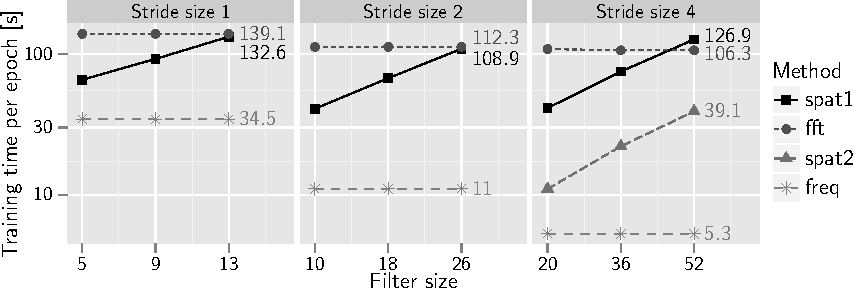
\includegraphics{figures/NECO-03-14-2099-Figure-2}
%\input{r_figures/runtime_imgnet_c3_bw}
}

\subfloat[Running times of training a second layer sconvRBM with
16, 32, and 64 channels (stride size 1).] {
\label{fig:run_imgnet_l2}
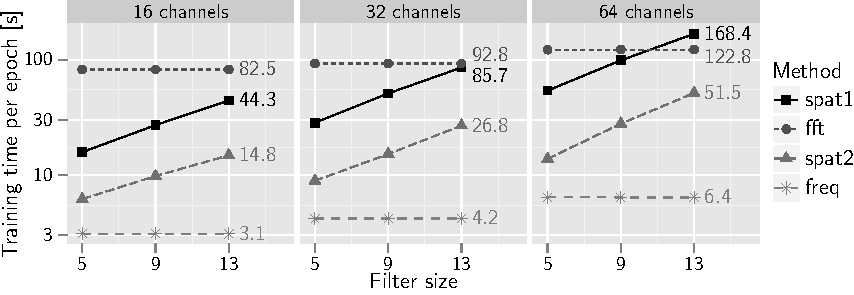
\includegraphics{figures/NECO-03-14-2099-Figure-3}
%\input{r_figures/runtime_imgnet_c16-64_bw}
}

\label{fig:run_imgnet}
\caption[Comparison of running times for training a sconvRBMs on 2D
images]{Comparison of running times for training a (a) first and (b) second
layer sconvRBM on 2D images using our frequency domain method (freq) and three
alternative methods using different convolution implementations: single image
convolutions (spat1), batched convolutions (spat2), and convolution by using
FFTs (fft). Due to internal limitations of the implementation of batched
convolutions, a comparison with spat2 could not be performed for images with a
resolution of \num{512x512} when using a stride size smaller than four.}
\end{figure}

Figure~\ref{fig:run_imgnet_l2} shows a similar comparison for training the
second convRBM layer for a stride size of 1 and varying filter sizes and numbers
of channels. In contrast to training the first layer, training times mostly
depend on the calculation of convolutions, where the impact of calculating
convolutions on the total running time increases with an increasing number of
channels. Training in the frequency domain is between 5 to 26 times faster than
training in the spatial domain using single-image convolutions, and 2
to 8 times faster than using batched convolutions. For all channel sizes,
batched training is about 3 to 4 times faster than non-batched training and
calculating convolutions using FFTs is much slower than batched training and
training in the frequency domain. To summarize, training of 2D images in the
frequency domain is much faster than training in the spatial domain even for
small filter sizes.
Using the largest filter kernels in both layers, the proposed method is shown to
yield a speedup of 7 to 8 times compared to state-of-the-art GPU
implementations.

\subsubsection{Running Time Analysis on 3D Volumes (OASIS)}

Figure~\ref{fig:run_oasis} shows the comparison of running times for training a
first  and second layer sconvRBM on 3D volumes for varying filter sizes, stride
sizes, and varying numbers of channels. In contrast to training on 2D images,
the computational costs of calculating 3D convolutions break even with
calculating FFTs for small filter sizes, because the number of multiplications
and additions per convolution increases cubically, instead of quadratically,
with the filter kernel size. As a result, simply training by convolutions in the
frequency domain is faster than in the spatial domain. However, our proposed
training algorithm still outperforms both other methods, even at the smallest
filter size. For filter sizes of 5 and larger, our frequency domain
implementation is between 3.5 to 200 times faster than our spatial domain
implementation using single-image convolutions and 2.7 to 17 times faster than
calculating convolutions by FFTs. Similar to the results on 2D images, training
times of the first layer using a stride of 1 depend strongly on the time
required to calculate the expectation of the hidden units and to sample the
hidden units. Hence, performance improvements of our frequency domain method are
more pronounced for larger strides and numbers of channels, where the impact of
calculating convolutions on the total training time is also larger. This makes
the proposed method particularly suitable for training sconvRBMs on
high-resolution 3D volumes.

\begin{figure}[t!]
\subfloat[Running times of training a first layer sconvRBM with stride sizes of 1, 2, and 4.] {
\label{fig:run_oasis_l1}
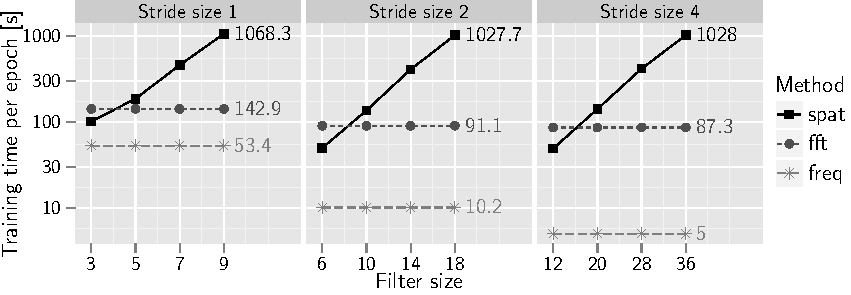
\includegraphics{figures/NECO-03-14-2099-Figure-4}
%\input{r_figures/runtime_oasis_c1_bw}
}

\subfloat[Running times of training a second layer sconvRBM with 8, 16, and 32
channels (stride size 1).] {
\label{fig:run_oasis_l2}
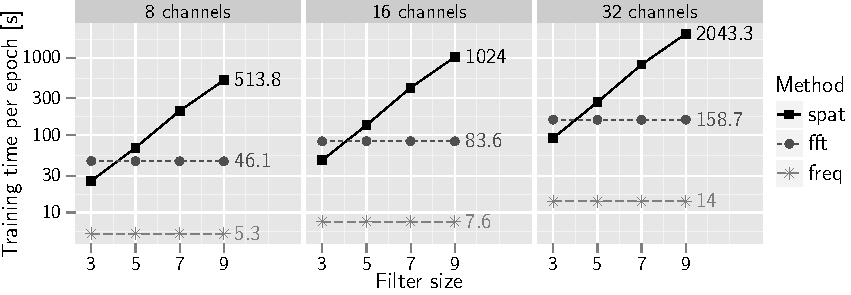
\includegraphics{figures/NECO-03-14-2099-Figure-5}
%\input{r_figures/runtime_oasis_c8-32_bw}
}
\caption[Comparison of running times for training a sconvRBMs on 3D
images]{Comparison of running times for training a (a) first and (b) second
layer sconvRBM on 3D volumes using a single 3D image convolution implementation
(spat), an implementation that calculates convolutions by using FFTs (fft), and
our proposed implementation in the frequency domain (freq).}
\label{fig:run_oasis}
\end{figure}

\section{Manifold of AD Patients}

% Motivation and short overview of the method and why use this one and not
% alternatives. What data was used? Applied to RAW MRI images without much
% preprocessing.

In this paper, we propose a novel approach for learning the manifold of brain
images that uses a deep belief network (DBN) \cite{Hinton2006b} to discover
patterns of similarity in groups of images. In contrast to previous
brain manifold learning algorithms, DBNs do not assume the manifold
space to be locally linear and do not require a previously defined similarity
measure or the construction of a proximity graph.
\begin{itemize}
\item DBNs mostly limited to 2D images, still the case?
\item Our fast training method allows DBNs to be used for manifold learning of
3D medical images
\end{itemize}

Contribution is the demonstration that DBNs can learn a low-dimensional manifold
of brain volumes that detects modes of variation that correlate to demographic
and disease parameters.

\subsection{Method}

% Explain the method in more detail. Also what tools where used for the
% experiments and stuff. How was the DBN designed and why.

% TODO: Less math an more model. Maybe draw the entire model in a figure or at
% least have a table with the parameters. Emphasise use of a strided
% convolutional RBM for dimensionality reduction

% TODO: Fuse this with the rest of the text. Look at MICCAI 2014 to know how.

We have evaluated the proposed method on a subset of the ADNI dataset
\cite{Petersen2010}, containing 300 T1-weighted MRIs of Alzheimer's disease (AD)
and normal subjects. The images were provided skull-stripped and bias field
corrected. We resampled all images to a resolution of \num{128x128x128} voxels
and a voxel size of \SI{2.0x2.0x2.0}{\milli\meter}. We then normalized their
intensities to a common range, and rigidly registered them to a group-wise mean
image prior to training and testing. We did not perform non-rigid registration
for spatial normalization in order to evaluate the capabilities of the method
without the added confound of complex registration parameters. The dataset was
divided into a training set and a test set such that each set contains 75 AD and
75 normal subjects. To learn the manifold of brain MRIs, we used a DBN with
three convRBM layers and two RBM layers. After three convRBMs, the dimension of
each image is reduced to \num{8x8x8} and small enough for RBMs. The training of
the DBN took approximately 43 hours on two GeForce GTX 560 Ti graphics cards.

Our proposed method performs manifold learning by reducing the dimensionality of
the input images using a DBN, a deep generative model that is composed of
multiple restricted Boltzmann machines (RBMs)~\cite{Hinton2006b} as illustrated
by the simplified example in Fig.~\ref{fig:rbmscheme}.
% TODO: No simplified model. The real model is needed.
An RBM is a Markov random
field with trainable weights whose nodes are divided into a visible layer
$\vect{v}$ representing the inputs of the model and a hidden layer $\vect{h}$
representing extracted features from the inputs. The first RBM receives the
intensity values of a group of images as input and reduces the dimensionality of
each image by discovering patterns of similarity that are common within groups
of images. Subsequent RBMs receive the hidden unit activations of the previous
RBM as input, thus learning successively more complex and abstract patterns from
a training set. The number of trainable weights increases significantly with the
resolution of the training images. In order to scale the model to
high-resolution images, the first several layers of our DBN are convolutional
RBMs (convRBMs), a type of RBM that uses weight sharing to reduce the number of
trainable weights, albeit at the cost of using the much more computationally
expensive convolutions instead of multiplications. In the remainder of this
section, we will briefly review the training of convRBMs, followed by a
description of our novel training algorithm that performs parameter learning in
frequency domain. For comprehensive introductions to RBMs and convRBMs, the
reader is referred to \cite{Hinton2006b} and \cite{Lee2011}, respectively.

Our algorithm for the dimensionality reduction of an input image using a
convRBM is illustrated in Fig.~\ref{fig:convrbm}. In contrast to previous work
that uses max pooling to reduce the dimensionality \cite{Lee2011}, all steps
involved in our method are invertible, which allows the reconstruction of
images from their manifold coordinates. In the first step, the pixels of an
input image are reorganized into multiple images of lower resolution in order to
reduce the dimensionality of a single image. The number of images in the image
vector is then reduced with the following steps.
To apply the model to real-valued data like the intensities of some medical
images, the visible units are modeled as Gaussian units. When the visible units have
been mean centered and standardized to unit variance, the expectation of the
visible units is given by
\begin{equation} 
\E[v_i \given \vect{h}] = \textstyle\sum_j w_{ij}*h_j + b_i
\label{eq:convvis}
\end{equation}
where $v_i, h_j, b_i \in \R^{N \times N \times N}$, $b_i$ are bias terms, $N$ is
the image size, $w_{ij} \in \R^{N_w \times N_w \times N_w}$ are the weights,
$N_w$ is the size of a weight kernel, and $*$ denotes circular convolution.
A binary hidden unit can only encode two states. In order to increase the
expressive power of the hidden units, we use noisy rectified
linear units as the hidden units,
which has shown to improve the learning performance~\cite{Nair2010} of RBMs.
The
hidden units can be sampled with
\begin{equation} 
h_j \sim \max(0, \mu_j + \Norm(0, \sigm(\mu_j)))
\label{eq:convhid}
\end{equation} 
where $\mu_j = \textstyle\sum_i\tilde{w}_{ij}*v_i +c_j$, $c_j \in \R^{N \times
N \times N}$, $\tilde{w}$ denotes a flipped version of $w$ in all three
dimensions, $\Norm(0, \sigma^2)$ denotes Gaussian noise, and $\sigm(x)$ is the
sigmoid function defined as $\sigm(x) = (1+ \exp(-x))^{-1}, x \in \R$. The
weights and bias terms of a convRBM can be learned using contrastive
divergence (CD) \cite{Hinton2006b}. During each iteration of the algorithm, the
gradient of the parameters is estimated and a gradient step with a fixed
learning rate is performed. The gradient of the weights can be approximated by:
\begin{equation}
\Delta w_{ij} = v_i*\tilde{h}_j - v_i'*\tilde{h}_j'
\label{eq:convgra}
\end{equation}
where $h_j$ and $h_j'$ are samples drawn from $p(h_j \given \vect{v})$ and
$p(h_j \given \vect{v}')$ using \eqref{eq:convhid} and $v_i' = \E[v_i \given
\vect{h}]$.

\subsection{Evaluation}

The geometric fit of the learned manifold model was evaluated in terms of the
generalizability to new images and the specificity to images from the training
set. The generalizability was measured as the average root mean squared error
(RMSE) between an image and its reconstruction, normalized by the intensity
range of the input image. The specificity was measured by calculating the
average RMSE between images randomly generated from the manifold model and the
most similar images from the training set. \ref{fig:genspe} shows a
comparison of the reconstruction errors between the training and test sets, and
the specificity at different layers of the DBN. The similarity of the
reconstruction errors between the training and test images indicates that no
overfitting is occurring. The average reconstruction error at the last layer is
below \SI{6}{\percent}. Even though the very small reconstruction error is
partially due to head MRIs having a large amount of homogeneous background, it
demonstrates the ability of the learned manifold to capture most of the visual
information with only two manifold parameters. The opposite slopes of the
reconstruction errors and error of generated images indicates a trade-off
between generalizability and specificity in the earlier phases of training. The
low errors at the end of training (Layer 5) indicates that the method is able to
be both specific and generalizable.

\begin{figure}[tb]
\centering
  % Created by tikzDevice version 0.6.2-92-0ad2792 on 2013-06-06 10:46:52
% !TEX encoding = UTF-8 Unicode
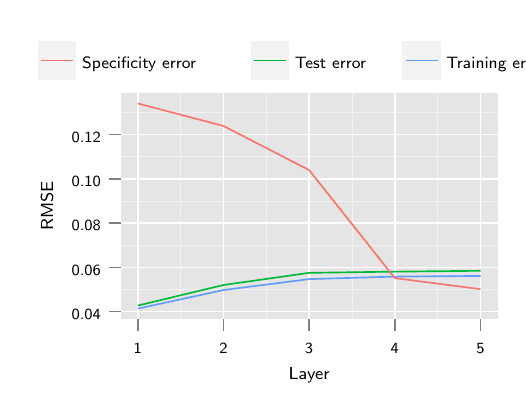
\begin{tikzpicture}[x=1pt,y=1pt]
\tikzstyle{clip}=[]
\definecolor[named]{fillColor}{rgb}{1.00,1.00,1.00}
\path[use as bounding box,fill=fillColor,fill opacity=0.00] (0,0) rectangle (169.83,130.09);
\begin{scope}
\path[clip] ( 33.55, 24.84) rectangle (169.83,106.43);
\definecolor[named]{fillColor}{rgb}{0.90,0.90,0.90}

\path[fill=fillColor] ( 33.55, 24.84) rectangle (169.83,106.43);
\definecolor[named]{drawColor}{rgb}{0.95,0.95,0.95}

\path[draw=drawColor,line width= 0.3pt,line join=round] ( 33.55, 35.47) --
	(169.83, 35.47);

\path[draw=drawColor,line width= 0.3pt,line join=round] ( 33.55, 51.46) --
	(169.83, 51.46);

\path[draw=drawColor,line width= 0.3pt,line join=round] ( 33.55, 67.46) --
	(169.83, 67.46);

\path[draw=drawColor,line width= 0.3pt,line join=round] ( 33.55, 83.45) --
	(169.83, 83.45);

\path[draw=drawColor,line width= 0.3pt,line join=round] ( 33.55, 99.44) --
	(169.83, 99.44);

\path[draw=drawColor,line width= 0.3pt,line join=round] ( 55.23, 24.84) --
	( 55.23,106.43);

\path[draw=drawColor,line width= 0.3pt,line join=round] ( 86.21, 24.84) --
	( 86.21,106.43);

\path[draw=drawColor,line width= 0.3pt,line join=round] (117.18, 24.84) --
	(117.18,106.43);

\path[draw=drawColor,line width= 0.3pt,line join=round] (148.15, 24.84) --
	(148.15,106.43);
\definecolor[named]{drawColor}{rgb}{1.00,1.00,1.00}

\path[draw=drawColor,line width= 0.6pt,line join=round] ( 33.55, 27.47) --
	(169.83, 27.47);

\path[draw=drawColor,line width= 0.6pt,line join=round] ( 33.55, 43.47) --
	(169.83, 43.47);

\path[draw=drawColor,line width= 0.6pt,line join=round] ( 33.55, 59.46) --
	(169.83, 59.46);

\path[draw=drawColor,line width= 0.6pt,line join=round] ( 33.55, 75.45) --
	(169.83, 75.45);

\path[draw=drawColor,line width= 0.6pt,line join=round] ( 33.55, 91.45) --
	(169.83, 91.45);

\path[draw=drawColor,line width= 0.6pt,line join=round] ( 39.75, 24.84) --
	( 39.75,106.43);

\path[draw=drawColor,line width= 0.6pt,line join=round] ( 70.72, 24.84) --
	( 70.72,106.43);

\path[draw=drawColor,line width= 0.6pt,line join=round] (101.69, 24.84) --
	(101.69,106.43);

\path[draw=drawColor,line width= 0.6pt,line join=round] (132.67, 24.84) --
	(132.67,106.43);

\path[draw=drawColor,line width= 0.6pt,line join=round] (163.64, 24.84) --
	(163.64,106.43);
\definecolor[named]{drawColor}{rgb}{0.38,0.61,1.00}

\path[draw=drawColor,line width= 0.6pt,line join=round] ( 39.75, 28.55) --
	( 70.72, 35.28) --
	(101.69, 39.23) --
	(132.67, 40.14) --
	(163.64, 40.37);
\definecolor[named]{drawColor}{rgb}{0.00,0.73,0.22}

\path[draw=drawColor,line width= 0.6pt,line join=round] ( 39.75, 29.66) --
	( 70.72, 37.10) --
	(101.69, 41.49) --
	(132.67, 41.93) --
	(163.64, 42.24);
\definecolor[named]{drawColor}{rgb}{0.97,0.46,0.43}

\path[draw=drawColor,line width= 0.6pt,line join=round] ( 39.75,102.72) --
	( 70.72, 94.58) --
	(101.69, 78.65) --
	(132.67, 39.60) --
	(163.64, 35.60);
\end{scope}
\begin{scope}
\path[clip] (  0.00,  0.00) rectangle (169.83,130.09);
\definecolor[named]{drawColor}{rgb}{0.00,0.00,0.00}

\node[text=drawColor,anchor=base east,inner sep=0pt, outer sep=0pt, scale=  0.80] at ( 26.44, 24.72) {0.04};

\node[text=drawColor,anchor=base east,inner sep=0pt, outer sep=0pt, scale=  0.80] at ( 26.44, 40.71) {0.06};

\node[text=drawColor,anchor=base east,inner sep=0pt, outer sep=0pt, scale=  0.80] at ( 26.44, 56.71) {0.08};

\node[text=drawColor,anchor=base east,inner sep=0pt, outer sep=0pt, scale=  0.80] at ( 26.44, 72.70) {0.10};

\node[text=drawColor,anchor=base east,inner sep=0pt, outer sep=0pt, scale=  0.80] at ( 26.44, 88.69) {0.12};
\end{scope}
\begin{scope}
\path[clip] (  0.00,  0.00) rectangle (169.83,130.09);
\definecolor[named]{drawColor}{rgb}{0.50,0.50,0.50}

\path[draw=drawColor,line width= 0.6pt,line join=round] ( 29.29, 27.47) --
	( 33.55, 27.47);

\path[draw=drawColor,line width= 0.6pt,line join=round] ( 29.29, 43.47) --
	( 33.55, 43.47);

\path[draw=drawColor,line width= 0.6pt,line join=round] ( 29.29, 59.46) --
	( 33.55, 59.46);

\path[draw=drawColor,line width= 0.6pt,line join=round] ( 29.29, 75.45) --
	( 33.55, 75.45);

\path[draw=drawColor,line width= 0.6pt,line join=round] ( 29.29, 91.45) --
	( 33.55, 91.45);
\end{scope}
\begin{scope}
\path[clip] (  0.00,  0.00) rectangle (169.83,130.09);
\definecolor[named]{drawColor}{rgb}{0.50,0.50,0.50}

\path[draw=drawColor,line width= 0.6pt,line join=round] ( 39.75, 20.58) --
	( 39.75, 24.84);

\path[draw=drawColor,line width= 0.6pt,line join=round] ( 70.72, 20.58) --
	( 70.72, 24.84);

\path[draw=drawColor,line width= 0.6pt,line join=round] (101.69, 20.58) --
	(101.69, 24.84);

\path[draw=drawColor,line width= 0.6pt,line join=round] (132.67, 20.58) --
	(132.67, 24.84);

\path[draw=drawColor,line width= 0.6pt,line join=round] (163.64, 20.58) --
	(163.64, 24.84);
\end{scope}
\begin{scope}
\path[clip] (  0.00,  0.00) rectangle (169.83,130.09);
\definecolor[named]{drawColor}{rgb}{0.00,0.00,0.00}

\node[text=drawColor,anchor=base,inner sep=0pt, outer sep=0pt, scale=  0.80] at ( 39.75, 12.22) {1};

\node[text=drawColor,anchor=base,inner sep=0pt, outer sep=0pt, scale=  0.80] at ( 70.72, 12.22) {2};

\node[text=drawColor,anchor=base,inner sep=0pt, outer sep=0pt, scale=  0.80] at (101.69, 12.22) {3};

\node[text=drawColor,anchor=base,inner sep=0pt, outer sep=0pt, scale=  0.80] at (132.67, 12.22) {4};

\node[text=drawColor,anchor=base,inner sep=0pt, outer sep=0pt, scale=  0.80] at (163.64, 12.22) {5};
\end{scope}
\begin{scope}
\path[clip] (  0.00,  0.00) rectangle (169.83,130.09);
\definecolor[named]{drawColor}{rgb}{0.00,0.00,0.00}

\node[text=drawColor,anchor=base,inner sep=0pt, outer sep=0pt, scale=  0.90] at (101.69,  3.01) {Layer};
\end{scope}
\begin{scope}
\path[clip] (  0.00,  0.00) rectangle (169.83,130.09);
\definecolor[named]{drawColor}{rgb}{0.00,0.00,0.00}

\node[text=drawColor,rotate= 90.00,anchor=base,inner sep=0pt, outer sep=0pt, scale=  0.90] at (  9.21, 65.64) {RMSE};
\end{scope}
\begin{scope}
\path[clip] (  0.00,  0.00) rectangle (169.83,130.09);
\definecolor[named]{fillColor}{rgb}{1.00,1.00,1.00}

\path[fill=fillColor] ( -4.49,106.76) rectangle (207.88,129.75);
\end{scope}
\begin{scope}
\path[clip] (  0.00,  0.00) rectangle (169.83,130.09);
\definecolor[named]{drawColor}{rgb}{1.00,1.00,1.00}
\definecolor[named]{fillColor}{rgb}{0.95,0.95,0.95}

\path[draw=drawColor,line width= 0.6pt,line join=round,line cap=round,fill=fillColor] (  3.39,111.03) rectangle ( 17.85,125.49);
\end{scope}
\begin{scope}
\path[clip] (  0.00,  0.00) rectangle (169.83,130.09);
\definecolor[named]{drawColor}{rgb}{0.97,0.46,0.43}

\path[draw=drawColor,line width= 0.6pt,line join=round] (  4.84,118.26) -- ( 16.40,118.26);
\end{scope}
\begin{scope}
\path[clip] (  0.00,  0.00) rectangle (169.83,130.09);
\definecolor[named]{drawColor}{rgb}{0.97,0.46,0.43}

\path[draw=drawColor,line width= 0.6pt,line join=round] (  4.84,118.26) -- ( 16.40,118.26);
\end{scope}
\begin{scope}
\path[clip] (  0.00,  0.00) rectangle (169.83,130.09);
\definecolor[named]{drawColor}{rgb}{0.97,0.46,0.43}

\path[draw=drawColor,line width= 0.6pt,line join=round] (  4.84,118.26) -- ( 16.40,118.26);
\end{scope}
\begin{scope}
\path[clip] (  0.00,  0.00) rectangle (169.83,130.09);
\definecolor[named]{drawColor}{rgb}{1.00,1.00,1.00}
\definecolor[named]{fillColor}{rgb}{0.95,0.95,0.95}

\path[draw=drawColor,line width= 0.6pt,line join=round,line cap=round,fill=fillColor] ( 80.31,111.03) rectangle ( 94.76,125.49);
\end{scope}
\begin{scope}
\path[clip] (  0.00,  0.00) rectangle (169.83,130.09);
\definecolor[named]{drawColor}{rgb}{0.00,0.73,0.22}

\path[draw=drawColor,line width= 0.6pt,line join=round] ( 81.76,118.26) -- ( 93.32,118.26);
\end{scope}
\begin{scope}
\path[clip] (  0.00,  0.00) rectangle (169.83,130.09);
\definecolor[named]{drawColor}{rgb}{0.00,0.73,0.22}

\path[draw=drawColor,line width= 0.6pt,line join=round] ( 81.76,118.26) -- ( 93.32,118.26);
\end{scope}
\begin{scope}
\path[clip] (  0.00,  0.00) rectangle (169.83,130.09);
\definecolor[named]{drawColor}{rgb}{0.00,0.73,0.22}

\path[draw=drawColor,line width= 0.6pt,line join=round] ( 81.76,118.26) -- ( 93.32,118.26);
\end{scope}
\begin{scope}
\path[clip] (  0.00,  0.00) rectangle (169.83,130.09);
\definecolor[named]{drawColor}{rgb}{1.00,1.00,1.00}
\definecolor[named]{fillColor}{rgb}{0.95,0.95,0.95}

\path[draw=drawColor,line width= 0.6pt,line join=round,line cap=round,fill=fillColor] (135.08,111.03) rectangle (149.54,125.49);
\end{scope}
\begin{scope}
\path[clip] (  0.00,  0.00) rectangle (169.83,130.09);
\definecolor[named]{drawColor}{rgb}{0.38,0.61,1.00}

\path[draw=drawColor,line width= 0.6pt,line join=round] (136.53,118.26) -- (148.09,118.26);
\end{scope}
\begin{scope}
\path[clip] (  0.00,  0.00) rectangle (169.83,130.09);
\definecolor[named]{drawColor}{rgb}{0.38,0.61,1.00}

\path[draw=drawColor,line width= 0.6pt,line join=round] (136.53,118.26) -- (148.09,118.26);
\end{scope}
\begin{scope}
\path[clip] (  0.00,  0.00) rectangle (169.83,130.09);
\definecolor[named]{drawColor}{rgb}{0.38,0.61,1.00}

\path[draw=drawColor,line width= 0.6pt,line join=round] (136.53,118.26) -- (148.09,118.26);
\end{scope}
\begin{scope}
\path[clip] (  0.00,  0.00) rectangle (169.83,130.09);
\definecolor[named]{drawColor}{rgb}{0.00,0.00,0.00}

\node[text=drawColor,anchor=base west,inner sep=0pt, outer sep=0pt, scale=  0.85] at ( 19.65,115.33) {Specificity error};
\end{scope}
\begin{scope}
\path[clip] (  0.00,  0.00) rectangle (169.83,130.09);
\definecolor[named]{drawColor}{rgb}{0.00,0.00,0.00}

\node[text=drawColor,anchor=base west,inner sep=0pt, outer sep=0pt, scale=  0.85] at ( 96.57,115.33) {Test error};
\end{scope}
\begin{scope}
\path[clip] (  0.00,  0.00) rectangle (169.83,130.09);
\definecolor[named]{drawColor}{rgb}{0.00,0.00,0.00}

\node[text=drawColor,anchor=base west,inner sep=0pt, outer sep=0pt, scale=  0.85] at (151.34,115.33) {Training error};
\end{scope}
\end{tikzpicture}


\caption[Generalizability vs. specificity of a DBN for different numbers of
layers]{Generalizability vs. specificity of a DBN for different numbers of
layers. The similarity of the reconstruction errors between the training and
test images indicates that no overfitting occurs. The opposite slopes of the reconstruction errors and error of generated images (specificity error)
indicates a trade-off between generalizability vs. specificity in the earlier
phases of training, but the low errors at Layer 5 indicate that the method is
both generalizable and specific.}
\label{fig:genspe}
\end{figure}

\begin{figure}[tb]
\centering
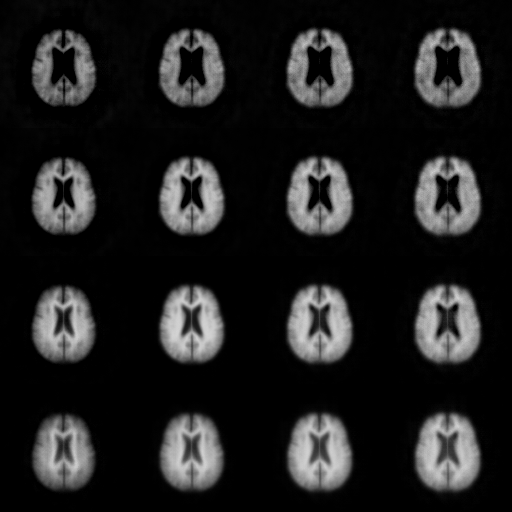
\includegraphics[width=0.3\textwidth, trim=0 -4em 0 0]
  {figures/MICCAI2013_sampled2d}

\caption[Axial slices from generated volumes from the manifold]{Axial slices
from generated volumes from the manifold. An increase of the first and second manifold dimension visually correlates with an increase in
brain and ventricle size, respectively.}
\label{fig:generated}
\end{figure}

Figure~\ref{fig:generated} shows axial slices of 16 volumes sampled at the
grid points of a 2D regular grid in manifold space. Volumes sampled along the
first manifold dimension (from left to right) appear to increase in brain size,
and the images sampled along the second manifold dimension (from bottom to top)
appear to increase in ventricle size. Figure~\ref{fig:scatter} shows an axial slice of
each image of the training set plotted against its manifold coordinates.
Consistent with images sampled from the manifold, an increase in ventricle size,
which is indicative of brain atrophy (a hallmark of AD), visually correlates
with an increase of the second manifold coordinate.
The AD/normal status is indicated by the frame color of each image. The vertical
separation between AD and normals suggests that the second manifold coordinate is
potentially of practical use in differentiating between AD and normal.

\begin{figure}[tb] \centering
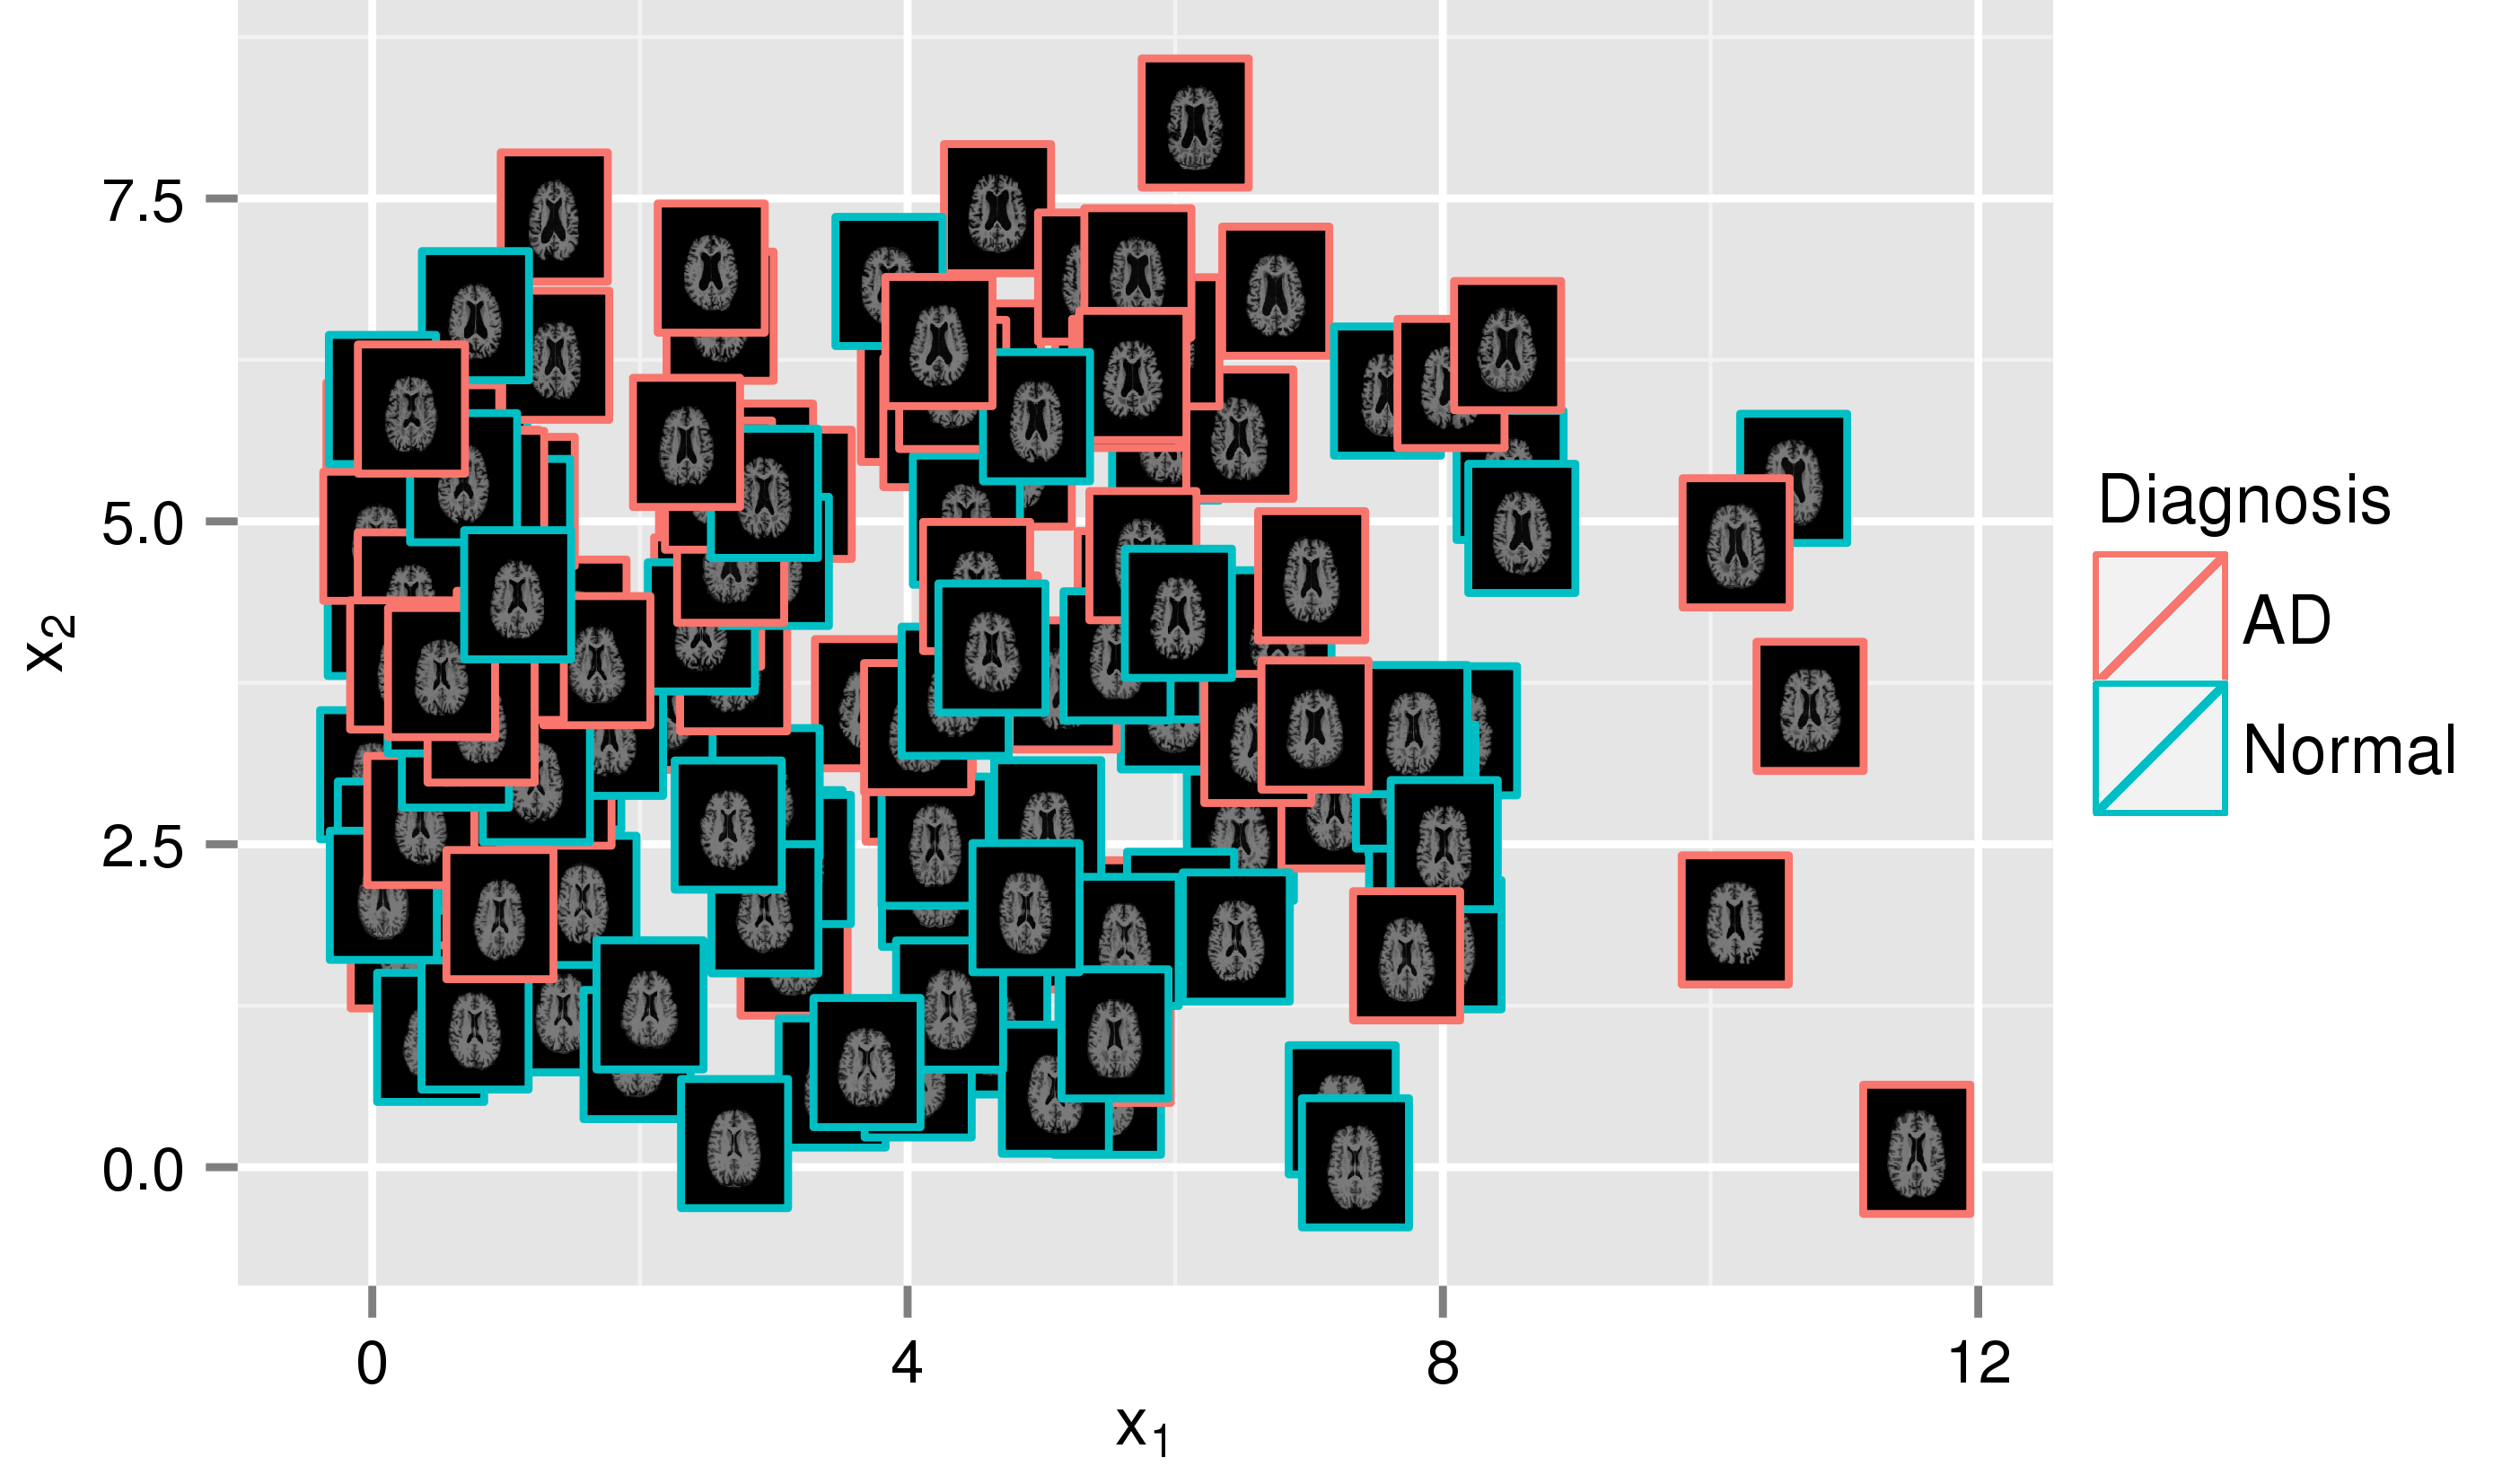
\includegraphics[width=0.75\textwidth]{figures/MICCAI2013_scatter3}
\caption[Axial slices of volumes from the training set plotted against their
manifold coordinates]{Axial slices of volumes from the training set plotted
against their manifold coordinates. The brains with larger ventricles, indicative of atrophy,
are mostly at the top, which is also where most of the AD patients are.}
\label{fig:scatter}
\end{figure}

To evaluate the potential of the manifold coordinates to reveal or predict
clinically relevant information, we have calculated the Pearson correlation $r$
of demographic parameters (age, gender) and disease parameters (mini-mental
state examination (MMSE) score, AD/normal status) with the manifold coordinates
($x_1$ and $x_2$). The results of the correlation tests are summarized in
Table~\ref{tab:corr}. Age, MMSE and AD/normal status show highly significant
correlations with $x_2$ ($p$-values between \num{9.85e-9} and \num{3.53e-7}),
which makes intuitive sense because $x_2$ visually correlates with ventricle
size. The first manifold coordinate correlates strongest with gender
($p\text{-value} = \num{8.24e-9}$), which also makes sense in terms of the
general difference in size between male and female. The strength and
significance of the correlations demonstrate the potential of deep learning of
brain images for classification and prediction of disease status.

\begin{table}[tb]
\small
\centering
\caption[Pearson correlation of demographic and clinical parameters with
manifold coordinates]{Pearson correlation $r$ of demographic and
clinical parameters with manifold coordinates ($x_1$, $x_2$). The stronger correlation in each column is
highlighted in bold.}
\sisetup{
  round-mode = places,
  round-precision = 2,
  exponent-product = \cdot,
  detect-weight=true,detect-inline-weight=math,
  tight-spacing = true
}%

\begin{tabular}{l*{4}{@{\hspace{15pt}}cc}}
\toprule
& \multicolumn{2}{c}{Age} & \multicolumn{2}{c}{Gender} &
\multicolumn{2}{c}{MMSE} & \multicolumn{2}{c}{AD/Normal Status} \\
& $r$ & $p$-value & $r$ & $p$-value & $r$ & $p$-value
& $r$ & $p$-value \\
\midrule
% V1
$x_1$ &
\num{-0.1734} & \num{0.03378} &
\textbf{\num{0.4490381}} & \textbf{\num{8.239e-09}} &
\num{0.0116499} & \num{0.8875} &
\num{-0.03231144} & \num{0.6947} \\
% V2
$x_2$ &
\textbf{\num{0.4469}} & \textbf{\num{9.848e-09}} &
\num{0.1860143} & \num{0.02266} &
\textbf{\num{-0.4015518}} & \textbf{\num{3.527e-07}} &
\textbf{\num{0.4127084}} & \textbf{\num{1.536e-07}} \\
\bottomrule
\end{tabular}
\label{tab:corr}
\end{table}


\section{Variability of Morphology and Lesion Distribution}

Multiple sclerosis (MS) is an inflammatory and degenerative disease of the
central nervous system with pathology that can be observed in vivo by magnetic
resonance imaging (MRI). MS is characterized by the formation of lesions,
primarily visible in white matter on conventional MRI, and the death of nervous
tissue leading to global and regional atrophy. A number of imaging biomarkers,
such as lesion volume and whole brain volume, have established their importance
for the study of MS. However, MS is a complex disease whose pathological
variability extends well beyond what can be captured by global and local
volumetric measures. Methods based on statistics of diffeomorphisms have been
used to discover patterns of regional atrophy \cite{Ceccarelli2012}, but they
are not designed to directly model morphological variability. It would be highly
desirable to have a method that can automatically discover potentially important
patterns of variability in brain morphology and lesion distribution, which would
advance our understanding of the complex pathology of MS. In addition, the joint
modeling of brain morphology and lesion distribution would further our knowledge
of how these two key pathological features interact. However, this type of
modeling is very challenging due to the high dimensionality of the data. In
recent years, there has been an increased interest in biomarker discovery using
manifold learning to form high-level representations of medical images
\cite{Wolz2010b,AljabarRueckert2011,Wolz2012}. Manifold learning is motivated by
the assumption that the space of brain images can be modeled to some
approximation by a low-dimensional manifold. Various methods for manifold
learning have been proposed (e.g., locally linear embedding (LLE), Laplacian
eigenmaps (LEM), Isomaps) \cite{Cayton2005}, with Isomaps and LEM being the most
popular for medical image analysis. Most such methods require a prebuilt
proximity graph based on a selected distance measure, the choice of which can be
crucial for manifold learning \cite{Gerber2010}. Aljabar et al. proposed a
method \cite{AljabarRueckert2011} for the joint modeling of multiple image
features of neonatal brains. First, separate manifolds based on features from
geometric surface models, non-rigid deformations, and image intensities are
learned, then a second dimensionality reduction step is used to combine the
individual manifold parameters.

We present a new method for modeling the variability in the morphology and
lesion distribution of a large set of MRIs of MS patients. Our method is built
using a deep belief network (DBN) \cite{Hinton2006b}, a layered network whose
parameters can be learned from training images. An advantage of DBNs over other
manifold learning methods is that it does not require a prebuilt proximity
graph, which is particularly beneficial for modeling lesions, because the
spareness and randomness of MS lesions make defining a suitable distance measure
challenging and potentially biasing. Instead, the DBN approach assumes that a
particular lesion configuration is a sample from an unknown distribution of
lesion configurations that can be parameterized by a relatively small set of
lesion distribution parameters. We model morphological and lesion variability
with two individual DBNs, then form a joint model by replacing the individual
top network layers with a new layer that joins both DBNs, similarly to the work
on the joint modeling of auditory and visual signals for speech recognition
\cite{Ngiam2011}. Our results show that this model can automatically discover
the classic patterns of MS pathology, as well as more subtle ones, and that the
distribution parameters computed are found to have strong relationships to MS
clinical scores.

% Short overview. New data. Deformation fields directly and lesion masks for MS.
% Motivation for that: correspondence but without eliminating variability in
% morphology. Why use deep learning and not another method for that?

\subsection{Method}

Our proposed model for pattern discovery consists of three main components (a) a
model that aims to find patterns of morphological changes in deformation fields,
(b) a model that aims to find patterns in the spatial distribution of lesions,
and (c) a joint model that aims to find concurring deformation and lesion
distribution patterns. The morphology model is learned from a set of
displacement fields that are calculated via non-rigid registration from a set of
T1-weighted (T1w) brain MRIs $D \subset I$, $I = \{I_n \mid I_n\colon\Omega
\mapsto \R$\}, $\Omega \subset \R^3$ and the ICBM 152 nonlinear atlas template
image \cite{Fonov2011}. First, all images of the training set are aligned to MNI
space by a 9 degree-of-freedom registration using FLIRT \cite{Jenkinson2002}.
Then for each image $I_n \in D$, the displacement field $u_n$, $u\colon \Omega
\mapsto \R^3$, that describes the non-rigid transformation from template
coordinates to image coordinates is calculated using FNIRT \cite{Andersson2007},
where the displacement field $u_n$ is represented by a \num{40x48x22} grid of 3D
displacement vectors. We assume that the displacement fields $u_n$ are samples
from an unknown distribution $p(u \mid D_1, \dotsc)$ that can be parameterized
by far fewer parameters than the dimensionality of the fields themselves. In
practice, the user typically selects the number of parameters to represent the
data being explored. The task of finding patterns is to discover the underlying
probability density function $p(u \mid D_1, \dotsc)$, where the parameters
$(D_1,\dotsc)^T$ represent the patterns of variability of the displacement field
distribution. This allows us to compare the morphology of two brains at a very
high level in terms of the distribution parameters of their displacement fields
$u_1$ and $u_2$ given by $\E[D_1,\dotsc \mid u_1]$ and $\E[D_1,\dotsc \mid
u_2]$. Furthermore, we can visualize the modes of morphological variability of
MS brain images, by sampling the space of displacement fields spanned by $(D_1,
\dotsc)^T$ by calculating the expectation $\E[u \mid D_1, \dotsc]$ for a range
of values for $(D_1, \dotsc)^T$.

\begin{figure}[tb]
\centering
\begin{tikzpicture}[scale=0.75]
\tikzstyle{every node}=[font=\sffamily\small, inner sep=3pt, align=center]
\tikzstyle{every pin}=[align=center,fill=white]
\tikzstyle{dbnlabel}=[font=\sffamily]
         
% Deformation field
        
\node[dbnlabel, rotate=90] at (-1.5,2.25) {Morphology DBN};
        
\begin{scope}[xshift=-20pt,yslant=0.63,xscale=0.4]

\node[transform shape,pin={[pin
distance=8]125:Displacement\\
field $u$}] (field) at (2,2)
{\includegraphics[width=4cm]{figures/deformation2.png}};

% \node[pin={[pin distance=0.6,overlay]93:Displacement\\
% field $u$}] at ($(field.north west)!0.1!(field.north east)$) {};

\end{scope}
         
% 3-channel input

\foreach \x in {0, 10, 20} {
\begin{scope}[xshift=\x pt]
%\ifnum\x=0
%\path
%\else
\draw[fill=white, fill opacity=0.75]
%\fi
  (0,0) coordinate(A\x) -- ++(90:4) coordinate (B\x) -- ++(30:2) coordinate
  (C\x) -- ++(-90:4) -- cycle;
  

% \begin{scope}[xshift=-50pt,yslant=0.63,xscale=0.4]  
% \node[transform shape,inner sep=0pt] at (2,2)
%   {\includegraphics[width=4cm]{deformation2.png}};
% \end{scope}
  
\draw (0,3)
   ++(30:0.25) \ifnum\x=20 coordinate (a1) \else -- +(0:10pt) +(0:0) \fi
-- ++(90:0.5)  \ifnum\x=20 coordinate (b1) \else -- +(0:10pt) +(0:0) \fi
-- ++(30:0.25) \ifnum\x=20 coordinate (c1) \else -- +(0:10pt) +(0:0) \fi
-- ++(-90:0.5) \ifnum\x=20 coordinate (d1) \else -- +(0:10pt) +(0:0) \fi
-- ++(210:0.25);
\end{scope}
}

%\node[below=4pt,xshift=-3pt] at (A0)  {$u_x$};
%\node[below=4pt] at (A10) {$u_y$};
%\node[below=4pt,xshift=3pt] at (A20) {$u_z$};

\node[pin={[pin distance=5pt]260:$u_x$}] at (A0)  {};
\node[pin={[pin distance=5pt]270:$u_y$}] at (A10)  {};
\node[pin={[pin distance=5pt]290:$u_z$}] at (A20)  {};

% Transition

\draw ($(a1)!0.5!(c1)$) ++(55pt,-5pt) coordinate (e1);
\draw (a1) -- (e1);
\draw (b1) -- (e1);
\draw (c1) --node[pin={[pin distance=1cm]40:Strided\\ convolution}] {} (e1);
\draw (d1) -- (e1);

% First layer hidden units

\foreach \x in {80,85,90,95,100,105} {
\begin{scope}[xshift=\x pt,yshift=1.5cm,scale=0.5]
\draw[fill=white, fill opacity=0.75]
  (0,0) coordinate(A\x) -- ++(90:4) coordinate (B\x) -- ++(30:2) coordinate
  (C\x) -- ++(-90:4) coordinate(D\x) -- cycle;
   
\draw (0,2.5)
   ++(30:0.25) \ifnum\x=105 coordinate (a2) \else -- +(0:10pt) +(0:0) \fi
-- ++(90:1)    \ifnum\x=105 coordinate (b2) \else -- +(0:10pt) +(0:0) \fi
-- ++(30:0.5)  \ifnum\x=105 coordinate (c2) \else -- +(0:10pt) +(0:0) \fi
-- ++(-90:1)   \ifnum\x=105 coordinate (d2) \else -- +(0:10pt) +(0:0) \fi
-- ++(210:0.5);
\end{scope}
}

\draw[decorate,decoration={brace,raise=20pt}] (B0|-C0) --node[above=25pt]
{Strided convolutional RBM} (C105|-C0);

\draw[decorate,decoration={brace,raise=4pt,mirror}]
%(A80) --node[below=8pt] {$N = 32$} (A80-|D105);
(A80) --node[below=8pt] {$N = 32$} (A80-|D105);

\draw ($(a2)!0.5!(c2)$) ++(0:38pt) coordinate (e2);
\draw (a2) -- (e2);
\draw (b2) -- (e2);
\draw (c2) -- (e2);
\draw (d2) -- (e2);

% Second layer hidden units

\foreach \x in {145, 150, ..., 175, 180} {
\begin{scope}[xshift=\x pt,yshift=2.25cm,scale=0.25]
\draw[fill=white, fill opacity=0.75]
  (0,0) coordinate(A\x) -- ++(90:4) coordinate (B\x) -- ++(30:2) coordinate
  (C\x) -- ++(-90:4) coordinate(D\x) -- cycle;
\draw (0,1.75)
   ++(30:0.25) \ifnum\x=180 coordinate (a3) \else -- +(0:20pt) +(0:0) \fi
-- ++(90:2)    \ifnum\x=180 coordinate (b3) \else -- +(0:20pt) +(0:0) \fi
-- ++(30:1)    \ifnum\x=180 coordinate (c3) \else -- +(0:20pt) +(0:0) \fi
-- ++(-90:2)   \ifnum\x=180 coordinate (d3) \else -- +(0:20pt) +(0:0) \fi
-- ++(210:1);
\end{scope}
}

\draw[decorate,decoration={brace,raise=4pt,mirror}]
(A145) --node[below=8pt] {$N = 64$} (A145-|D180);

\draw ($(a3)!0.5!(c3)$) ++(0:18pt) coordinate (e3);
\draw (a3) -- (e3);
\draw (b3) -- (e3);
\draw (c3) -- (e3);
\draw (d3) -- (e3);

% Third layer hidden units

\foreach \x in {200, 205, ..., 240} {
\begin{scope}[xshift=\x pt,yshift=2.625cm,scale=0.125]
\draw[fill=white, fill opacity=0.75]
  (0,0) coordinate(A\x) -- ++(90:4) coordinate (B\x) -- ++(30:2) coordinate
  (C\x) -- ++(-90:4) coordinate(D\x) -- cycle;
\end{scope}
}

% Forth layer visible units (dense)

\begin{scope}[xshift=280pt, yshift=2.75cm]
\foreach \x/\y in {0/-2, 1/-1.5, 2/-1, 3/-0.5, 4/0, 5/0.5, 6/1, 7/1.5, 8/2} {
  \node[circle, draw] (v\x) at (0,\y) {};
}
\end{scope}

\draw[shorten >=10pt,shorten <=10pt,dashed] (A240)--(v0.south west);
\draw[shorten >=10pt,shorten <=10pt,dashed] (A240|-C240)--
node[label=120:Vectorize\\ hidden units] {} (v8.north west);

\draw[decorate,decoration={brace,raise=4pt,mirror}]
(A200) --node[below=8pt,fill=white] {$N = 32$} (A200-|D240);

%\node[rotate=90,fill=white,align=center] at(270pt,2.75cm) {Serialize\\ hidden
%units};

% Forth layer hidden units (dense)

\begin{scope}[xshift=320pt, yshift=2.75cm]
\foreach \x/\y in {0/-1, 1/-0.5, 2/0, 3/0.5, 4/1} {
  \node[circle, draw] (h\x) at (0,\y) {};
}
\end{scope}

\foreach \x in {0, ..., 8} {
  \foreach \y in {0, ..., 4} {
    \draw[very thin] (v\x)--(h\y);
  }
}

\draw[decorate,decoration={brace,raise=20pt}] (v8.west|-C0)
--node[above=25pt] {Dense RBM} (h0.east|-C0);

% Fifth layer hidden units (distribution parameters)

\begin{scope}[xshift=360pt, yshift=2.75cm]
\foreach \x/\y in {1/0.25, 2/-0.25} {
  \node[circle, draw, label=0:$D_\x$] (D\x) at (0,\y) {};
}
\end{scope}

\foreach \x in {0, ..., 4} {
  \foreach \y in {1,2} {
    \draw[very thin] (h\x)--(D\y);
  }
}

% \draw[decorate,decoration={brace,raise=22pt}]
% (D1.north-|D1.east) --node[above,sloped] {Deformation\\ parameters}
% (D2.south-|D2.east);

%%%%%%%%%%%%%%%%%%%%%
% Lesion Model
%%%%%%%%%%%%%%%%%%%%%

\begin{scope}[yshift=-6cm]

\node[dbnlabel, rotate=90] at (-1.5,2.25) {Lesion DBN};

\begin{scope}[xshift=-25pt,yslant=0.63,xscale=0.4] 
\node[transform shape,pin={[pin distance=15]140:Lesion\\
mask $l$}] at (2,2)
  {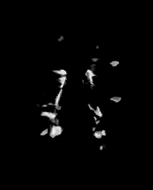
\includegraphics[height=4cm]{figures/lesions.png}};
\end{scope}

% 1-channel input

\foreach \x in {20} {
\begin{scope}[xshift=\x pt]
\draw[fill=white, fill opacity=0.75]
  (0,0) coordinate(A\x) -- ++(90:4) coordinate (B\x) -- ++(30:2) coordinate
  (C\x) -- ++(-90:4) coordinate (D\x) -- cycle;
  
\draw (0,3)
   ++(30:0.25) \ifnum\x=20 coordinate (a1) \else -- +(0:10pt) +(0:0) \fi
-- ++(90:0.5)  \ifnum\x=20 coordinate (b1) \else -- +(0:10pt) +(0:0) \fi
-- ++(30:0.25) \ifnum\x=20 coordinate (c1) \else -- +(0:10pt) +(0:0) \fi
-- ++(-90:0.5) \ifnum\x=20 coordinate (d1) \else -- +(0:10pt) +(0:0) \fi
-- ++(210:0.25);
\end{scope}
}

\node[pin=30:Visible\\ units] at ($(C20)!0.25!(D20)$) {};

% Transition

\draw ($(a1)!0.5!(c1)$) ++(55pt,-5pt) coordinate (e1);
\draw (a1) -- (e1);
\draw (b1) -- (e1);
\draw (c1) -- (e1);
\draw (d1) -- (e1);

% First layer hidden units

\foreach \x in {80,85,90,95,100,105} {
\begin{scope}[xshift=\x pt,yshift=1.5cm,scale=0.5]
\draw[fill=white, fill opacity=0.75]
  (0,0) coordinate(A\x) -- ++(90:4) coordinate (B\x) -- ++(30:2) coordinate
  (C\x) -- ++(-90:4) coordinate(D\x) -- cycle;
   
\draw (0,2.5)
   ++(30:0.25) \ifnum\x=105 coordinate (a2) \else -- +(0:10pt) +(0:0) \fi
-- ++(90:1)    \ifnum\x=105 coordinate (b2) \else -- +(0:10pt) +(0:0) \fi
-- ++(30:0.5)  \ifnum\x=105 coordinate (c2) \else -- +(0:10pt) +(0:0) \fi
-- ++(-90:1)   \ifnum\x=105 coordinate (d2) \else -- +(0:10pt) +(0:0) \fi
-- ++(210:0.5);
\end{scope}
}

\draw[decorate,decoration={brace,raise=4pt,mirror}]
%(A80) --node[below=8pt] {$N = 32$} (A80-|D105);
(A80) --node[below=8pt] {$N = 32$} (A80-|D105);

\draw ($(a2)!0.5!(c2)$) ++(0:38pt) coordinate (e2);
\draw (a2) -- (e2);
\draw (b2) -- (e2);
\draw (c2) -- (e2);
\draw (d2) -- (e2);

\node[pin=30:Hidden\\ units] at ($(C105)!0.2!(D105)$) {};

% Second layer hidden units

\foreach \x in {145, 150, ..., 175, 180} {
\begin{scope}[xshift=\x pt,yshift=2.25cm,scale=0.25]
\draw[fill=white, fill opacity=0.75]
  (0,0) coordinate(A\x) -- ++(90:4) coordinate (B\x) -- ++(30:2) coordinate
  (C\x) -- ++(-90:4) coordinate(D\x) -- cycle;
\draw (0,1.75)
   ++(30:0.25) \ifnum\x=180 coordinate (a3) \else -- +(0:20pt) +(0:0) \fi
-- ++(90:2)    \ifnum\x=180 coordinate (b3) \else -- +(0:20pt) +(0:0) \fi
-- ++(30:1)    \ifnum\x=180 coordinate (c3) \else -- +(0:20pt) +(0:0) \fi
-- ++(-90:2)   \ifnum\x=180 coordinate (d3) \else -- +(0:20pt) +(0:0) \fi
-- ++(210:1);
\end{scope}
}

\draw[decorate,decoration={brace,raise=4pt,mirror}]
(A145) --node[below=8pt] {$N = 64$} (A145-|D180);

\draw ($(a3)!0.5!(c3)$) ++(0:18pt) coordinate (e3);
\draw (a3) -- (e3);
\draw (b3) -- (e3);
\draw (c3) -- (e3);
\draw (d3) -- (e3);

% Third layer hidden units

\foreach \x in {200, 205, ..., 240} {
\begin{scope}[xshift=\x pt,yshift=2.625cm,scale=0.125]
\draw[fill=white, fill opacity=0.75]
  (0,0) coordinate(A\x) -- ++(90:4) coordinate (B\x) -- ++(30:2) coordinate
  (C\x) -- ++(-90:4) coordinate(D\x) -- cycle;
\end{scope}
}

%\node[rotate=90] at(270pt,2.75cm) {Serialize hidden units};

% Forth layer visible units (dense)

\begin{scope}[xshift=280pt, yshift=2.75cm]
\foreach \x/\y in {0/-2, 1/-1.5, 2/-1, 3/-0.5, 4/0, 5/0.5, 6/1, 7/1.5, 8/2} {
  \node[circle, draw] (V\x) at (0,\y) {};
}
\end{scope}

\draw[shorten >=10pt,shorten <=10pt,dashed] (A240)--(V0.south west);
\draw[shorten >=10pt,shorten <=10pt,dashed] (A240|-C240)--
%node[label=120:Vectorize\\ hidden units] {}
(V8.north west);

\draw[decorate,decoration={brace,raise=4pt,mirror}]
(A200) --node[below=8pt,fill=white] {$N = 32$} (A200-|D240);

%\node[rotate=90,fill=white,align=center] at(270pt,2.75cm) {Serialize\\ hidden
%units};

% Forth layer hidden units (dense)

\begin{scope}[xshift=320pt, yshift=2.75cm]
\foreach \x/\y in {0/-1, 1/-0.5, 2/0, 3/0.5, 4/1} {
  \node[circle, draw] (H\x) at (0,\y) {};
}
\end{scope}

\foreach \x in {0, ..., 8} {
  \foreach \y in {0, ..., 4} {
    \draw[very thin] (V\x)--(H\y);
  }
}

% Fifth layer hidden units (distribution parameters)

\begin{scope}[xshift=360pt, yshift=2.75cm]
\foreach \x/\y in {1/0.25, 2/-0.25} {
  \node[circle, draw, label=0:$L_\x$] (L\x) at (0,\y) {};
}
\end{scope}

\foreach \x in {0, ..., 4} {
  \foreach \y in {1,2} {
    \draw[very thin] (H\x)--(L\y);
  }
}
\end{scope}

%%%%%%%%%%%%%%
% Joint layer
%%%%%%%%%%%%%%

% yshift = 2.75 - 6/2 = -0.25

\begin{scope}[xshift=380pt, yshift=-0.25cm]
\foreach \x/\y in {1/-0.75, 2/-0.25, 3/0.25, 4/0.75} {
  \node[circle, draw, label=0:$J_\x$] (J\x) at (0,\y)
  {}; }
\end{scope}

\foreach \x in {0, ..., 4} {
  \foreach \y in {1, ..., 4} {
    \draw[very thin] (h\x)--(J\y);
    \draw[very thin] (H\x)--(J\y);
  }
}

\node[yshift=-15pt, fill=white, inner sep=3pt] at (h0) {$N = 16$};

\draw[decorate,decoration={brace,raise=30pt,mirror}] (V0.south-|J1)
--node[dbnlabel, below=35pt, sloped] {Joint DBN} (v8.north-|J1);

\end{tikzpicture}
\caption{DBN models used for discovering patterns.}
\end{figure}

The probability density function $p(u)$ is modeled by a deep belief network
(DBN) \cite{Hinton2006b}, a generative probabilistic graphical model consisting
of one layer of observed random variables (visible units) and multiple layers of
latent random variables (hidden units). In a DBN, each pair of adjacent layers
of random variables form a restricted Boltzmann machine (RBM). The first RBM
receives the displacement fields of a training set as input and reduces the
dimensionality of each field by discovering patterns of similarity that are
common within groups of displacement fields. Each subsequent RBM receives the
hidden unit activations of the previous RBM as input, thus learning successively
more complex and abstract patterns from the training data. In particular, we use
a DBN with three strided convolutional RBMs\footnote{The three sconvRBMs have
stride sizes of \num{2x2x1}, \num{2x2x2}, \num{1x1x1}, filter sizes of
\num{10x10x7}, \num{10x10x10}, \num{3x5x3}, and 32, 64, 32 filters,
respectively.} (sconvRBMs) and two dense RBMs \cite{Hinton2010} with 16 and 2
hidden units, respectively. In the following, we will briefly review the
sconvRBM, as this model is less often described in the literature, followed by
how the visible and hidden units of the DBN relate to displacement fields and
displacement field distribution parameters. A sconvRBM is a type of RBM in which
the probabilistic relationships between the visible and hidden units are
expressed in terms of strided convolutions, a type of convolution that shifts
the filter kernel as a sliding window with a step size or stride $s > 1$. Due to
the much smaller number of trainable parameters compared to dense RBMs,
sconvRBMs are best suited for learning low- to mid-level features from very
high-dimensional data. Compared to other more commonly used convolution-based
RBMs \cite{Lee2009}, an advantage of sconvRBMs is that inference is invertible,
which allows the reconstruction of the visible units from the hidden unit
activations. In our application, this would allow for the reconstruction of
deformation fields from distribution parameters. The complete morphology DBN can
be trained layer-by-layer by training each RBM individually using contrastive
divergence \cite{Hinton2006b}. Once the parameters of the DBN have been learned
from training data, we can use the model for inference. Let
$\vect{v}_{\text{d},1}, \dotsc, \vect{v}_{\text{d},5}$, $\vect{h}_{\text{d},1},
\dotsc, \vect{h}_{\text{d},5}$, and $\thetas_{\text{d},1}, \dotsc,
\thetas_{\text{d},5}$ denote the visible units, hidden units, and parameters,
respectively, of each RBM of the morphology DBN. Then, for a given displacement
field $u_n$, we can calculate the parameters $(D_1, \dotsc)^T$ of $u \sim p(u
\mid D_1, \dotsc)$ with
\begin{align} 
\label{eq:inferd}
(D_1, \dotsc)^T &= \E[D_1, \dotsc \mid u_n] = \E[\vect{h} \mid
\vect{v}_{\text{d},5}, \thetas_{\text{d},5}] \\
\label{eq:inferv}
\vect{v}_{\text{d},i+1} &= \E[\vect{h} \mid \vect{v}_{\text{d},i},
\thetas_{\text{d},i}]
\end{align}
where $i \in [1,4]$ and $\vect{v}_{\text{d},1} = u_n$. Inversely, the mean
displacement field $\bar{u}$ given the distribution parameters can be calculated
by
\begin{align}
\label{eq:inferu}
\bar{u} &= \E[u \mid D_1, \dotsc] = \E[\vect{v} \mid \vect{h}_{\text{d},1},
\thetas_{\text{d},1}] \\
\label{eq:inferh}
\vect{h}_{\text{d},i} &= \E[\vect{v} \mid \vect{h}_{\text{d},i+1},
\thetas_{\text{d},i+1}]
\end{align}
where $i \in [1,4]$ and $\vect{h}_{\text{d},5} = (D_1,\dotsc)^T$.

The input into our lesion model is a set of 3D binary lesion masks $l_n
\in I$, which have been created from T2-weighted (T2w) and PD-weighted (PDw) MRIs by experts using a semi-automatic method. All lesion masks are spatially aligned to MNI space using
the transformations as calculated for the corresponding T1w images. Analogous to
the morphology model, we assume that lesion masks $l_n$ are samples from
an unknown distribution $l_n \sim p(l \mid L_1, \dotsc)$ that can be
parameterized by only relatively few parameters $(L_1, \dotsc)^T$. The task of finding lesion
patterns is to discover the underlying probability density function $p(l \mid
L_1, \dotsc)$, where the parameters $(L_1, \dotsc)^T$ represent patterns of
variability of MS lesions. Similar to the morphology DBN, the lesion DBN
consists of three sconvRBMs\footnote{The three sconvRBMs have stride sizes of
\num{4x4x2}, \num{2x2x2}, \num{2x2x2}, filter sizes of \num{20x20x10},
\num{14x14x10}, \num{10x14x6}, and 32, 64, 64 filters, respectively.} and two
dense RBMs with 16 and 2 hidden units, respectively.
However, we modified the energy function of the sconvRBMs to account for the
sparse activation of MS lesion masks. Large black regions without local
structure can lead to random activations of the hidden units and consequently
the learning of random filters. To overcome this problem, we propose to
incorporate a region of interest (ROI) term into the energy equation of the
sconvRBM, which allows constraining the filter learning process to a given ROI.
This can be achieved by element-wise multiplication of the visible and hidden
units with a binary mask, which sets the visible and hidden units outside of the
ROI to zero, thereby removing their contribution to the energy of the model.
The ROI was chosen to include all white matter lesions from the training set.
Similarly to the morphology model, for a trained lesion DBN and a given lesion
mask $l_n$, we can calculate the parameters $(L_1,\dotsc)^T$ of $l_n \sim
p(l\mid L_1,\dotsc)$ in the same manner as in \eqref{eq:inferd} and
\eqref{eq:inferv}. Likewise, the mean lesion configuration $\bar{l}$ given the
distribution parameters $(L_1,\dotsc)^T$ can be calculated in the same manner as
in \eqref{eq:inferu} and \eqref{eq:inferh}.

To discover concurring patterns of morphology and lesion distribution, we
combine the morphology DBN and the lesion DBN to form the joint DBN, which
defines the joint distribution $p(u, l \mid J_1, \dotsc)$. The joint DBN
consists of two pathways, each corresponding to the first 4 layers of the
morphology and lesion DBNs, respectively, and a 5th RBM layer with 4 hidden
units, which replaces the 5th layer of the individual DBNs and combines the
hidden unit activations of the 4th layer RBMs. That is, the 5th RBM defines the
joint probability $p(\vect{v}_\text{j}, \vect{h}_\text{j} \mid
\thetas_\text{j})$, where $\vect{v}_\text{j} = (\vect{h}_{\text{d},4}^T,
\vect{h}_{\text{l},4}^T)^T$ and $\vect{h}_\text{j} = (J_1, \dotsc)^T$ are the
modes of variability of morphological and lesion distribution changes.


\subsection{Evaluation}

The proposed method was evaluated on a dataset from an MS clinical trial of 474
secondary progressive MS patients. For each subject, the dataset contains one
T1w, T2w, and PDw MRI with a resolution of \num{256x256x50} voxels and a voxel
size of \SI{0.937x0.937x3.000}{\milli\meter}. The main preprocessing steps
included rigid registration, brain extraction, intensity normalization, and
background cropping. We then trained the 3 DBN models as described in
Sect.~\ref{sec:method}.

The invertibility of our model allows the reconstruction of images from the
distribution parameters to visualize the discovered patterns of variability.
Figure~\ref{fig:deformations} shows axial slices from volumes generated from the
2-parameter morphology model $p(u \mid D_1, D_2)$. To generate these images, we
calculated the mean displacement fields for varying values of $D_1$ and $D_2$
to span the range of variability represented by the
training set and applied the inverse deformations to the ICBM 152 template
image. The most apparent morphological variability captured by the morphology
model is ventricular enlargement for $D_1$ and overall brain size for $D_2$.
Figure~\ref{fig:lesions} shows axial slices from the mean lesion configurations
$\E[l \mid L_1, L_2]$ for varying lesion distribution parameters. An increase of
$L_2$ visually correlates with an increase of lesions specifically around the
ventricles, whereas an increase of $L_1$ visually correlates with an increase of
lesions in the entire white matter.

\begin{figure}[tb]
\newlength{\subfigwidth}
\setlength{\subfigwidth}{0.232\textwidth}
\centering
\subfloat[Morphology manifold] {
\label{fig:deformations}
\begin{tikzpicture}
\tikzstyle{every node}+=[font=\scriptsize]
\node
(manifold){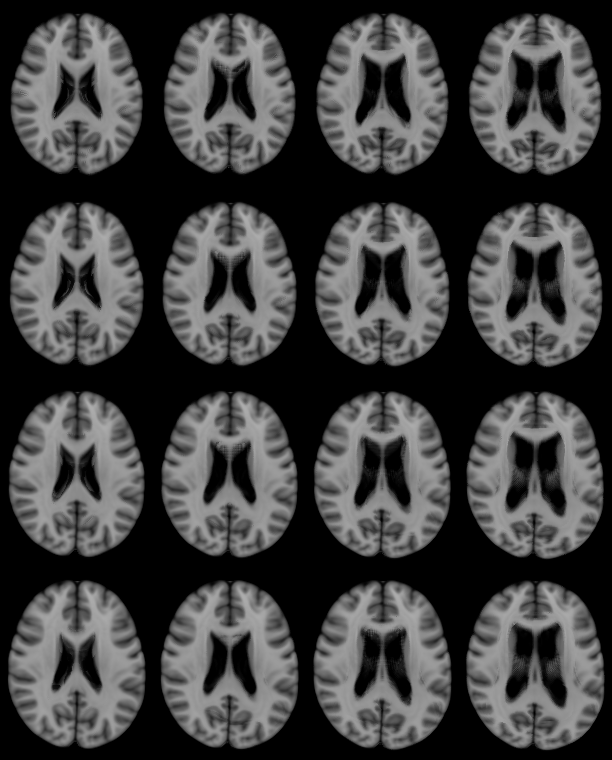
\includegraphics[width=\subfigwidth]{figures/MICCAI2014_warps_t1_dark}};

\draw[->] (manifold.south west)--node[below=4pt,inner sep=0] {$D_1$}
(manifold.south east);
\draw[->] (manifold.south west)--node[above=4pt,sloped,inner sep=0] {$D_2$}
(manifold.north west);

\end{tikzpicture}
}
\subfloat[Lesion manifold] {
\label{fig:lesions}
\begin{tikzpicture}
\tikzstyle{every node}+=[font=\scriptsize]
\node
(manifold){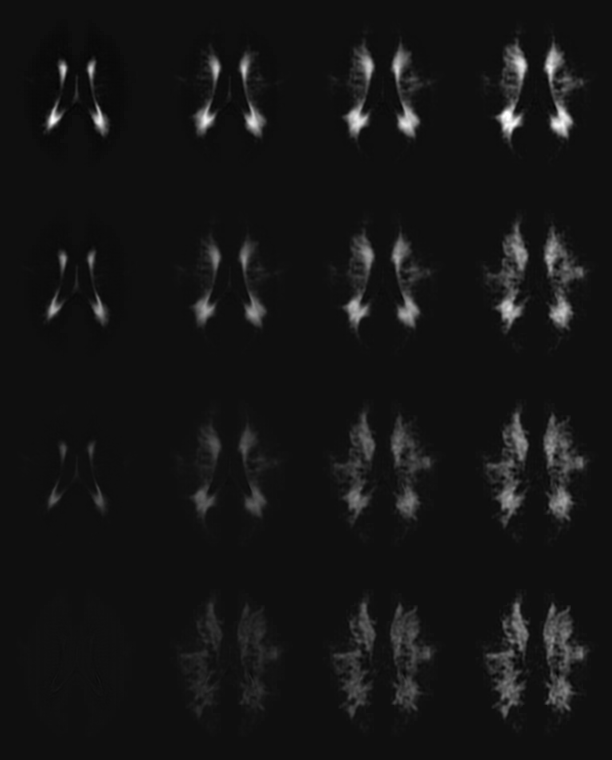
\includegraphics[width=\subfigwidth]{figures/MICCAI2014_p442_d0_full_h16-2}};

\draw[->] (manifold.south west)--node[below=4pt,inner sep=0] {$L_1$} (manifold.south east);
\draw[->] (manifold.south west)--node[above=4pt,sloped,inner sep=0] {$L_2$}
(manifold.north west);

\end{tikzpicture}
}%
\subfloat[Joint manifold] {
\label{fig:joint}
\begin{tikzpicture}
\tikzstyle{every node}+=[font=\scriptsize]

\node[align=left,fill=black,inner sep = 0pt] (manifold1) {
  \mbox{}\\[2pt]
  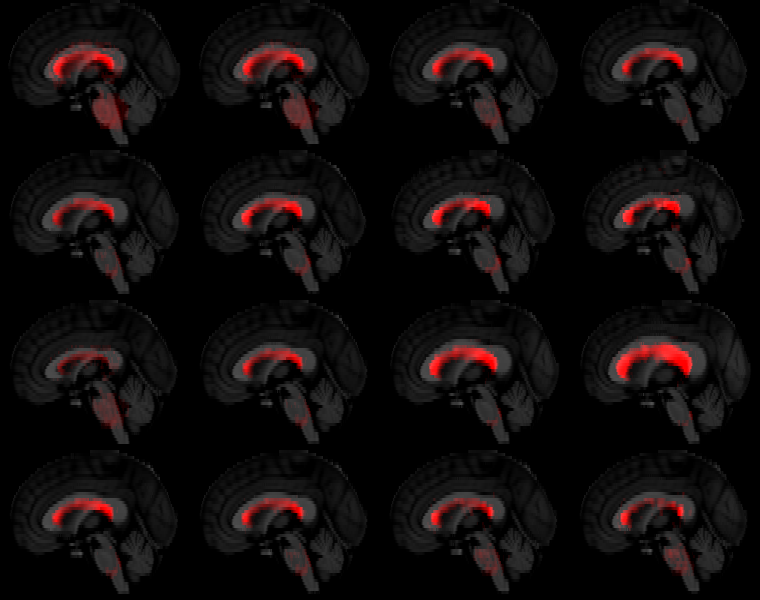
\includegraphics[trim=0 340 0 0,clip,width=\subfigwidth]
    {figures/MICCAI2014_full_rl1_h4_sag}\\[8.5pt]
  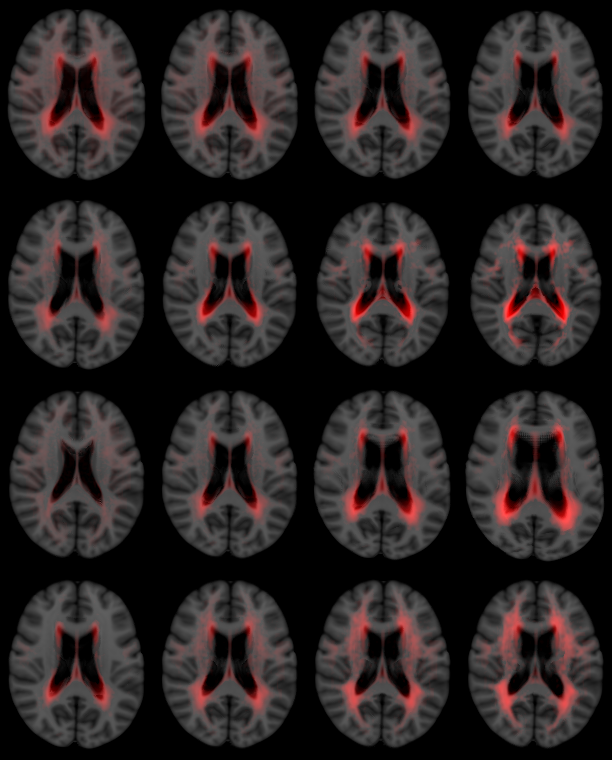
\includegraphics[trim=0 0 0 150,clip,width=\subfigwidth]
    {figures/MICCAI2014_full_rl1_h4}
};
\node[fit=(manifold1)] (manifold) { };

\foreach \x/\y in {0.125/1, 0.375/2, 0.625/3, 0.875/4} {
  \node[left,inner sep=0pt] at ($(manifold.north west)!\x!(manifold.south
  west)$) {$J_\y$}; }

\draw[->] (manifold.south west)--node[below=4pt,inner sep=0] {$J_x$} (manifold.south east);

\end{tikzpicture}
} \caption[Slices from generated volumes from the morphology, lesion,
and joint model]{Slices from generated volumes from the (a) morphology, (b)
lesion, and (c) joint model. The morphology model captures ventricular
enlargement ($D_1$) and decrease in brain size ($D_2$) as the main modes of
variation. For the lesion model, $L_1$ captures an increase in lesion load
throughout the WM, while $L_2$ captures primarily periventricular lesion load
variations. The parameters of the joint model capture combinations
of the variability found in the individual models.}
\label{fig:samples}
\end{figure}

To visualize concurring patterns of morphology and lesion distribution, we
sampled images from the joint model $p(u, l \mid J_1, \dotsc, J_4)$ as shown in
Fig.~\ref{fig:joint}. The images are deformed template images with superimposed
lesion masks. For each row, we varied only one distribution parameter and set
the remaining parameters to their mean values. Of the 4 parameters, $J_3$
visually corresponds most closely to the ``classic'' progression of MS
pathology, with an enlargement of the ventricles paired with an increased
periventricular lesion load. The parameters $J_2$ and $J_4$ also reveal
simultaneous morphological and lesion variations that are visible on the chosen
axial slice. For $J_1$, a lesion pattern is not obvious unless the images are
viewed sagittally, which reveals changes in lesion load in the pons.

\begin{table}[tb]
\centering 
\small

\caption[Pearson correlations of clinical scores with distribution parameters
and imaging biomarkers]{Pearson correlations $r$ of clinical scores with
distribution parameters of the morphology model ($D_1$, $D_2$), lesion model ($L_1$, $L_2$), joint model ($J_1$, $J_2$, $J_3$, $J_4$), normalized brain volume (nBV), and
lesion load (LL). The level of statistical significance is indicated by the
number of asterisks (* $p < 0.05$, ** $p < 0.01$, *** $p < 0.001$).
}

%\NewDocumentCommand{\sym}{m}{#1}

\label{tab:correlations}
\sisetup{
  round-mode = places,
  round-precision = 3,
  exponent-product = \cdot,
  detect-weight=true,
  detect-inline-weight=math,
  tight-spacing = false,
  table-align-text-post = false
}%

\def\tabspace{14pt}

\begin{tabular}{c@{\hspace{\tabspace}}c%
@{\hspace{\tabspace}}S[table-format=2.5]%
@{\hspace{\tabspace}}S[table-format=2.6]
@{\hspace{\tabspace}}S[table-format=2.6]
@{\hspace{\tabspace}}S[table-format=2.6]}
\toprule
 &  & {T25W} & {9-HPT} & {PASAT} & {MSFC} \\
 \midrule
 
\multirow{4}*{\minitab[c]{Individual\\ models}}
 & $D_1$ &
\bfseries -0.128976787246536** & -0.214588136146619*** & -0.282044527648157*** &
-0.314633263656368*** \\
 & $D_2$ & 0.0870255979372807 & 0.115835195120173* & 0.08923208653141 &
0.138616500875685** \\
& $L_1$ & -0.0581629511079419 & -0.231012897586838*** & -0.391822792658197*** &
-0.366992537420278*** \\
& $L_2$ & -0.091057480388512 & \bfseries -0.354478789398171*** &
\bfseries -0.426543205964196*** & \bfseries -0.463860459137063*** \\
\addlinespace
\multirow{4}*{\minitab[c]{Joint\\ model}}
 & $J_1$ & 0.107219513748914* & 0.285812780188632*** & 0.336253511146623*** &
0.378889115681159*** \\
 & $J_2$ & -0.037731447660239 & -0.209982769437628*** & -0.226800472678912***
& -0.255585426983655*** \\
& $J_3$ & \bfseries -0.117780586822506* & \bfseries -0.369169927947271*** &
\bfseries -0.452556545437486*** & \bfseries -0.494130959187706*** \\
& $J_4$ & -0.0491209563011896 & -0.205764640863705*** & -0.382954826511733*** &
-0.345529171963859*** \\
\addlinespace
\multirow{2}*{\minitab[c]{Imaging\\ biomarkers}}
 & nBV & 0.0530068558456253 & 0.143905618421747** & 0.246833144651129***
& 0.234774254053599*** \\
 & LL & -0.073681606595365 & \bfseries -0.286360084620956*** &
\bfseries -0.399646128024074*** & \bfseries -0.406222020153583*** \\
  
 \bottomrule
\end{tabular}

\end{table}

To evaluate the potential of the distribution parameters to reveal clinically
relevant information, we have calculated the Pearson correlation $r$ of the
clinical MS Functional Composite (MSFC) \cite{Fischer1999} and its components
(Timed 25-Foot Walk, T25W; 9-Hole Peg Test, 9-HPT; Paced Auditory Serial
Addition Test, PASAT) with the distribution parameters and two established MS
imaging biomarkers (normalized brain volume, nBV, as calculated by SIENAX
\cite{Smith2002} and lesion load, LL). The results of the correlation tests are
summarized in Table~\ref{tab:correlations}. In the individual models, all
parameters correlate significantly with 9-HPT, PASAT, and MSFC, except for $D_2$
with PASAT. The morphology parameter $D_1$ correlates more strongly with these
scores than nBV, as does the lesion parameter $L_2$ than LL. For T25W, $D_1$
shows a modest but significant correlation while nBV does not. In the joint
model, all parameters correlate significantly with 9-HPT, PASAT, and MSFC, with
$J_3$ being particularly strong. The parameter $J_3$ shows stronger correlations
than nBV or LL for all clinical scores, including a modest significant
correlation to T25W, which is not shown by nBV nor LL. The significant
correlation between $J_1$ and T25W is particularly interesting because the
lesion changes modeled by $J_1$ occur in the pons, which is known to be of
clinical significance for mobility. Overall, the learned parameters correlate
better than the established imaging biomarkers.

\begin{figure}[tb]
\centering
\subfloat[Morphological changes] {
\begin{tikzpicture} 
\tikzstyle{every node}=[font=\scriptsize]
\node[align=left,inner sep=0] (images) {
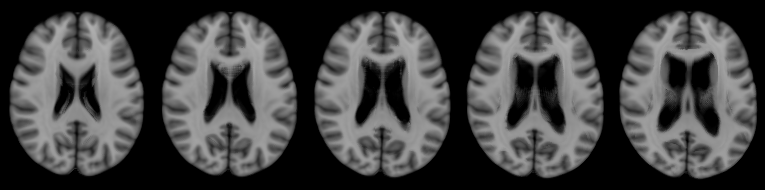
\includegraphics[width=0.47\textwidth]{figures/MICCAI2014_full_rl1_h4_MSFC_nolesion}
\\
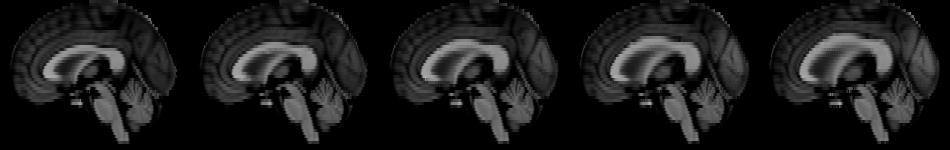
\includegraphics[width=0.47\textwidth]{figures/MICCAI2014_full_rl1_h4_MSFC_sag_nolesion}
};
\foreach \x/\y in {0.1/1.5, 0.3/0, 0.5/-1.5, 0.7/-3, 0.9/-4.5} {
  \node[above=2pt] at ($(images.north west)!\x!(images.north east)$) {\y}; }
\end{tikzpicture}
}
\subfloat[Lesion changes] {
\begin{tikzpicture}
\tikzstyle{every node}=[font=\scriptsize] 
\node[align=left,inner sep=0] (images) {
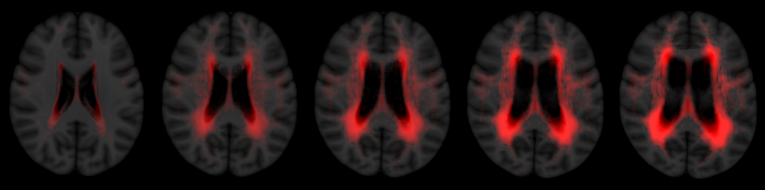
\includegraphics[width=0.47\textwidth]{figures/MICCAI2014_full_rl1_h4_MSFC} \\
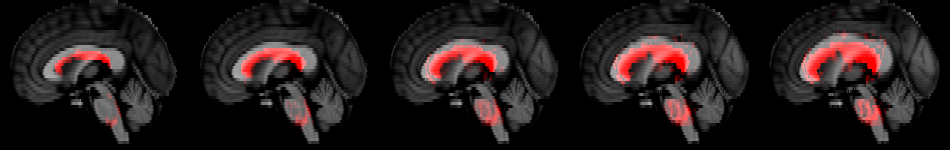
\includegraphics[width=0.47\textwidth]{figures/MICCAI2014_full_rl1_h4_MSFC_sag}
};
\foreach \x/\y in {0.1/1.5, 0.3/0, 0.5/-1.5, 0.7/-3, 0.9/-4.5} {
  \node[above=2pt] at ($(images.north west)!\x!(images.north east)$) {\y};
}
\end{tikzpicture}
}
\caption[Axial and mid-sagittal slices of volumes representing the spectrum of
MSFC scores]{Axial (top row) and mid-sagittal (bottom row) slices of volumes
representing the spectrum of MSFC scores from \num{1.5} to \num{-4.5}. A
decrease in MSFC shows the classic pattern of MS pathology.}
\label{fig:msspectrum}
\end{figure}

Another benefit of our model is the ability to visualize the progression of a
``mean'' secondary progressive MS brain along a range of MSFC scores.
To demonstrate, we trained 4 independent linear models to predict the
distribution parameters $J_1, \dotsc, J_4$ given the MSFC ($J_i = a_i +
b_i\text{MSFC}$). Figure~\ref{fig:msspectrum} shows the axial (top row) and
mid-sagittal (bottom row) slices of generated images representing the range of
MSFC scores from \num{1.5} to \num{-4.5}. Consistent with previous results, a
decrease in MSFC visually correlates with an increase in the size of the
ventricles, an increase in periventricular lesions, and an increase in lesions
in the pons region.

\section{Discussion}

Potentially follow up with a discussion where I can discuss related approaches
that came afterwards and what needs to be done.
